\chapter{Tools and Methods}
\label{ch:tools}

\fixme{Per Jon: This should cover simulation and reconstruction, tools and methods, and possibly calibration (Anne)}

%%%%%%%%%%%%%%%%%%%%%%%%%%%%%%%%%%%%%%%%%%%%%%%%%%%%%%%%%%%%%%%%
\section{Monte Carlo simulations}
\label{sec:tools-mc}

%Liquid argon time projection chambers (LArTPCs) provide a robust and elegant method for measuring the properties of neutrino interactions above a few tens of MeV by providing 3D event imaging with excellent spatial and energy resolution. For simulations, we produce large samples of Monte Carlo events (Monte Carlo Challenge - MCC) on a regular basis. The purpose is to test the latest simulation and reconstruction chain as well as the grid job submission tools and sam/tape interfaces and provide standard samples for various physics working groups to analyze. All the MCC samples are produced using the batch tool larbatch~\cite{ref:larbatch}.

%MCC1.0 was produced in January 2015 with three 35t samples. We include far detector and protoDUNE samples in later MCCs and incorporate more sophisticated detector simulation and reconstruction software. A more recent MC production MCC6.0, which was produced in May 2016, consists of 50 samples using the 35t, far detector and protoDUNE single-phase geometries. MCC6.0 was produced using LArSoft v05\_09\_01. The locations of the samples can be found in Ref~\cite{ref:mcc6}. 



Many physics processes are simulated in the DUNE far detector, which include beam neutrinos, atmospheric neutrinos, supernova neutrinos, proton decays and cosmogenic events. Figure~\ref{fig:dune_tpc} shows a portion of the DUNE single-phase TPC consisting of Anode Plane Assembly (APA) and Cathode Plane Assembly (CPA).

\begin{figure}[!ht]
\centering
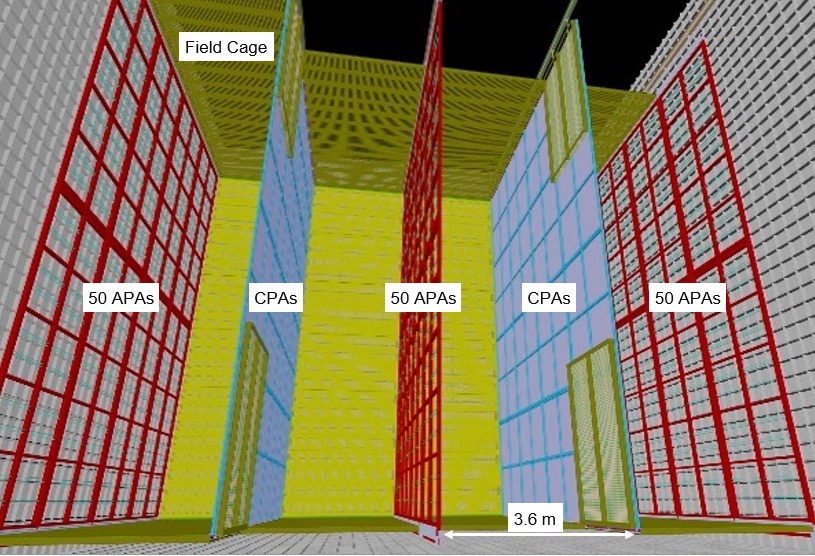
\includegraphics[width=0.7\textwidth]{DUNE_TPC.PNG}
\caption{A portion of DUNE single-phase TPC is shown. Four separate drift regions are separated by APA and CPA. }
\label{fig:dune_tpc}
\end{figure}

%In MCC6.0, we simulated 3 types of beam neutrinos (unoscillated $\nu_\mu$'s, fully-oscillated $\nu_{e}$'s and fully-oscillated $\nu_\tau$'s), atmospheric neutrinos, supernova neutrinos, proton decays and cosmogenic events in the far detector. 
In order to save processing time, all the far detector samples except the cosmogenics sample were simulated using a smaller version of the full 10-kt far detector geometry. This geometry is 13.9 m long, 12 m high and 13.3 m wide, which consists of 12 APAs and 24 TPCs. %In the default configuration, the TPC wire spacing is 5 mm, the wire angle is 36$^{\circ}$ and the neutrino beam is parallel to the wire planes. 
Figure~\ref{fig:dune_apa} shows the detailed structure of APA. %We also generated special samples where the wire spacing is 3 mm or the wire angle is 45$^{\circ}$ or the neutrino beam is perpendicular to the wire planes for the detector optimization studies. 

\begin{figure}[!ht]
\centering
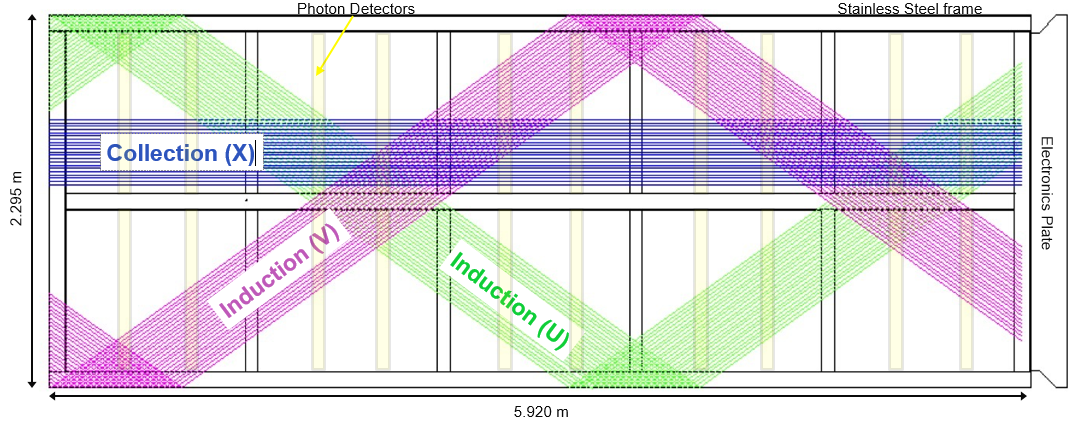
\includegraphics[width=0.7\textwidth]{DUNE_APA.PNG}
\caption{The detailed structure of the APA is shown. Each APA consists of four wrapped induction wire planes and two collection wire planes.
The photon detector is sandwiched between the two collection wire planes.}
\label{fig:dune_apa}
\end{figure}

For the simulation chain, each sample is simulated in 3 steps: generation (gen), {\sc geant4} tracking (g4), TPC signal simulation, and digitization (detsim). The first step is unique for each sample while the second and the third steps are mostly identical for all samples. 

%%%%%%%%%%%%%%%%%%%%%%%%%%%%%%%
\subsection{Hadron production and Beam Line modeling}
\label{sec:tools-mc-had-beam}

Currently described in the LBL chapter.

%\subsubsection{Key Properties of the LBNF Neutrino Beam}
%\label{ss:tools-beam-properties}

%\subsubsection{Modeling of Hadron Production from the Target}
%\label{ss:tools-hadron-production-modeling}

%\subsubsection{Modeling of LBNF Beam Line}
%\label{ss:tools-beam-line-modeling}

%%%%%%%%%%%%%%%%%%%%%%%%%%%%%%%
\subsection{Neutrino interaction generators} 
\label{sec:tools-mc-gen}

%\begin{itemize}
%\item Have this section owned by a Genie expert. Costas?
%\end{itemize}

%Both the beam neutrinos and atmospheric neutrinos were simulated using {\sc genie} v2\_10\_6. The beam neutrinos were simulated using the reference flux. We simulated unoscillated samples in both the neutrino and antineutrino modes. We also simulated fully oscillated samples where we convert all $\nu_\mu$'s in the beam to either $\nu_e$'s or $\nu_\tau$'s. 

%The atmospheric neutrinos were simulated using the Bartol flux for the Soudan site~\cite{ref:bartol}. There is a plan to use the Honda flux for the Homestake site~\cite{ref:honda} when the {\sc genie} flux interface is updated. 

\subsubsection{Supernova neutrinos}

The supernova neutrino events were generated using custom code wrapped in a LArSoft module.
This code simulates charged-current $\nu_e$-$^{40}$Ar interactions.
For each electron neutrino it calculates probabilities to produce a $^{40}$K nucleus
in different excited states (using a model from~\cite{Bhattacharya:1998hc}),
randomly selects one, and (with energy levels from~\cite{Cameron:2004myb}) 
produces several deexcitation $\gamma$s and an electron carrying the remaining energy.
All particles are produced isotropically,
there is no delay between the electron and corresponding deexcitation $\gamma$s
(in this model the $^{40}$K nucleus deexcites instantaneously) and they share a vertex,
which is simulated with equal probability anywhere in the active volume.
The primary neutrino energy distribution used in these samples is the cross-section-weighted 
energy spectrum obtained from SNOwGLoBES~\cite{snowglobes} (using the ``GKVM'' flux~\cite{GKVM}).
The supernova neutrino generator also allows to simulate a Poisson-distributed random number 
of neutrino interactions per event. These samples were simulated with, on average, 2 or 20 neutrinos.
In addition, one of the samples was generated with $1.01$~Bq/kg of $^{39}$Ar background.

\subsubsection{GENIE}

The DUNE Monte Carlo simulation chain is interfaced to the GENIE Event Generator \cite{Andreopoulos:2009rq}. This is an open-source product of the GENIE Collaboration [www.genie-mc.org] that provides state-of-the-art modelling of neutrino-nucleus interactions, as well as simulation of several other non-neutrino processes (nucleon decay, neutron-antineutron oscillation, boosted dark matter interactions, hadron and charged lepton scattering off nuclei). The Generator product also includes off-the-shelf components (flux drivers / interfaces to outputs of detailed neutrino beam-line simulations, detector geometry drivers, and several specialised event generation applications) for the simulation of realistic experimental setups. The GENIE Collaboration performs an advanced global analysis of neutrino scattering data, and is leading the development and characterization of comprehensive interaction models. The GENIE comprehensive models and physics tunes which are developed using its proprietary Comparisons and Tuning products, are fully integrated in the GENIE Generator product. Finally, the open-source GENIE Reweight product provides means for propagating modelling uncertainties. 

Building a comprehensive model for the simulation of neutrino interactions in the energy range of interest to current and near-future experiments poses significant challenges. This broad energy range bridges the perturbative and non-perturbative pictures of the nucleon and a variety of scattering mechanisms are important. In many areas, including elementary cross sections, hadronization models, and nuclear physics, one is required to piece together models with different ranges of validity in order to generate events over all of the available phase space. This inevitably introduces challenges in merging and tuning models, making sure that double counting and discontinuities are avoided. In addition, there are kinematic regimes which are outside the stated range of validity of all available models, in which case we are left with the challenge of developing our own models or deciding which model best extrapolates into this region. 

At the time of writing this document, Generator v3.0.0 was the most recent version released by the GENIE Collaboration [(1) Paper on GENIE3 in progress -- Will provide reference ASAP]. This version includes several new, state-of-the-art comprehensive models and tunes, whose performance against a large collection of neutrino, charged-lepton and hadron scattering data was characterised in detail [(2) Paper with detailed model characterization in progress -- Will provide reference ASAP]. The following comprehensive models and tunes are currently available:

{\bf G00\_00a\_00\_000} and {\bf G00\_00b\_00\_000}: They are equivalent to the historical ``Default'' and``Default+MEC'' models, as they were implemented in the latest releases of the v2 series of the GENIE Generator. They are empirical comprehensive models, based on home-grown hadronic simulations (AGKY model \cite{Yang:2009zx} for neutrino-induced hadronization and INTRANUKE/hA model \cite{Dytman:2015taa} for hadronic re-interactions) and nuclear neutrino cross-sections calculated within the framework of the simple Relativistic Fermi Gas model \cite{Bodek:1981wr}. Several processes are simulated within that framework with the most important ones, in terms of the size of the corresponding cross-section at few-GeV, being: a) quasi-elastic scattering, simulated using an implementation of the Llewellyn Smith model \cite{LlewellynSmith:1971uhs}, b) multi-nucleon interactions, simulated with an empirical model motivated by the Lightbody model \cite{Lightbody:1988gcu} and using a nucleon cluster model for the simulation of the hadronic system, c) baryon resonance neutrino-production simulated using an implementation of the Rein-Sehgal model \cite{Rein:1980wg}, and d) deep-inelastic scattering, simulated using the model of Bodek and Yang \cite{Bodek:2002ps}.  These comprehensive models, as well as the GENIE procedure for tuning the cross-section model in the transition region, have been used for several years and are well understood and documented \cite{Andreopoulos:2009rq}. The actual tune used is the one produced for the analysis of data from the MINOS experiment and, as it was already known at that time, it has several caveats as it emphasises inclusive data and does not address tensions with exclusive data. These comprehensive models and tunes are now unsupported, as they are superseded by the substantially improved versions listed below. However, they are included in v3 as they provide a connection with a large body of neutrino interaction studies.

{\bf G18\_01a\_02\_11a} and {\bf G18\_01b\_02\_11a}: They are adiabatically improved versions of the historical comprehensive models. They include new processes (diffractive production of pions, hyperon production) and major upgrades to the final-state hadronic re-interaction models (the `01a' version uses the INTRANUKE/hA2018 hadronic re-interaction model, whereas `01b' uses the INTRANUKE/hN2018 model) [(1) Paper on GENIE3 in progress], but leave the base cross-section model unchanged with respect to the historical model. However, the cross-section model was re-tuned to deuterium data and shows much improved agreement with several exclusive $1\pi$ and $2\pi$ channels, while it maintained good agreement with inclusive data. [(3) Paper on tunes in progress -- Will provide reference ASAP]

{\bf G18\_02a\_02\_11a} and {\bf G18\_02b\_02\_11a}: They are improved empirical models that share many of the features of G18\_01a\_02\_11a and G18\_01b\_02\_11a (new processes, improved hadronic simulations, new tunes), but introduced changes to the base cross-section model. In these comprehensive models, the Rein-Sehgal coherent and resonance neutrino-production models \cite{Rein:2006di, Rein:1980wg} were replaced with the better-motivated models produced by Berger-Sehgal \cite{Berger:2008xs, Berger:2007rq}.

{\bf G18\_10a\_02\_11a} and {\bf G18\_10b\_02\_11a}: They are comprehensive models anchored on the best theory currently impleented in GENIE. They are similar to G18\_02a\_02\_11a and G18\_02b\_02\_11a, respectively, but for the simulation of quasielastic-like processes they implement a modern microscopic calculation by the Valencia group. Quasi-elastic processes, within a Local Fermi Gas (LFG) model and simulating Coulomb and Random Phase Approximation (RPA) corrections are implemented based on Ref. \cite{Nieves:2004wx}, whereas 2p2h processes are implemented based on Ref. \cite{Nieves:2011pp}.

{\bf G18\_10i\_00\_000} and {\bf G18\_10j\_00\_000}: They are similar to G18\_10a\_02\_11a and G18\_10b\_02\_11a, but using the better-motivated $z$-expansion \cite{Hill:2010yb} of the axial form factor. However, due to extra complications in incorporating deuterium experiment flux constraints when using the $z$-expansion model in the GENIE tunes, both of these comprehensive models were untuned in v3.0.0, though a tune will be made available in a future revision. 

Besides simulation of of neutrino-nucleus interactions, GENIE provides simulation of several BSM physics channels:

{\bf Boosted Dark Matter}: The implementation of a boosted dark matter Monte Carlo simulation has been motivated by several theory studies \cite{Agashe:2014yua, Berger:2014sqa, Kong:2014mia, Cherry:2015oca, Kopp:2015bfa, Necib:2016aez, Alhazmi:2016qcs, Kim:2016zjx}. The current implementation focuses on two models presented in Ref \cite{Berger:2014sqa}. The first has a fermionic dark matter candidate, a $Z^\prime$ mediator, and a $u^0$ velocity dependence of the spin-dependent cross-section in the non-relativistic limit. The second model has a scalar dark matter candidate, a $Z^\prime$ mediator, and a $u^2$ velocity dependence of the spin-dependent cross-section in the non-relativistic limit.

{\bf Nucleon-decay}: GENIE simulates several nucleon decay topologies, using the exact same modelling of the initial nuclear state environment and intranuclear hadron transport as for the neutrino event simulation. In the nucleon decay simulation, the nucleon binding and momentum distribution is simulated using one of the nuclear models implemented in GENIE (typically a Fermi Gas model), and it is decayed to one of many topologies using a phase space decay. The decay products are produced within the nucleus and further re-interactions of hadrons are simulated by the GENIE hadron transport models. The simulated nucleon decay topologies are given in Table \ref{tbl:genie_ndk}.

{\bf Neutron-antineutron oscillation}: GENIE simulates several event topologies that may emerge following the annihilation of the antineutron produced from a bound neutron to antineutron transition. The simulation, as in the case of nucleon decay, uses the same modelling of the initial nuclear state environment and intranuclear hadron transport as for the neutrino event simulation. The simulated topologies are given in Table \ref{tbl:genie_antineutron}.

\begin{table}
  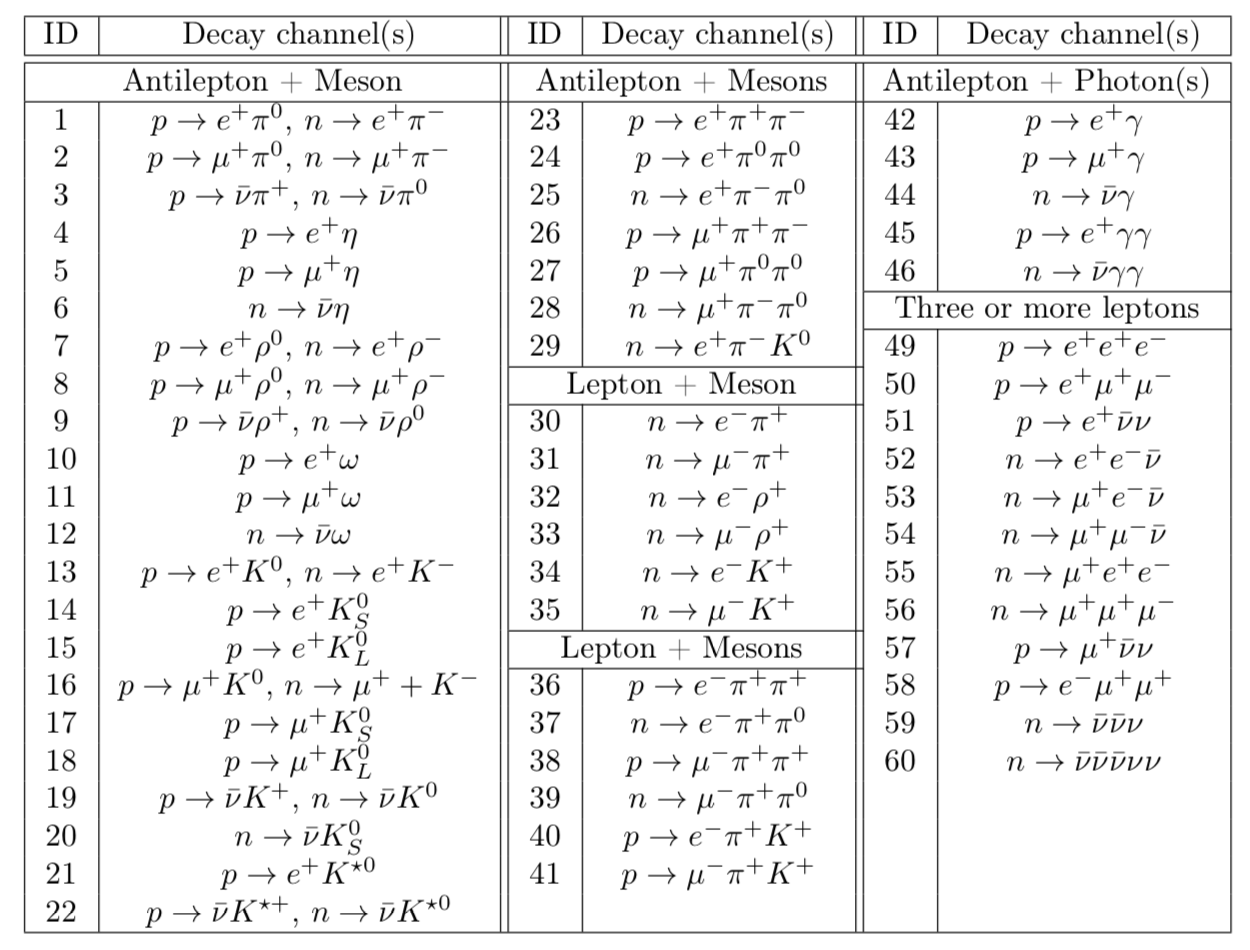
\includegraphics[width=\linewidth]{costas_table1}
  
  \caption[GENIE nucleon decay topologies]{Decay topologies considered in GENIE nucleon decay simulation. TODO: replace raster version}
  \label{tbl:genie_ndk}
\end{table}

\begin{table}
	\begin{centering}
		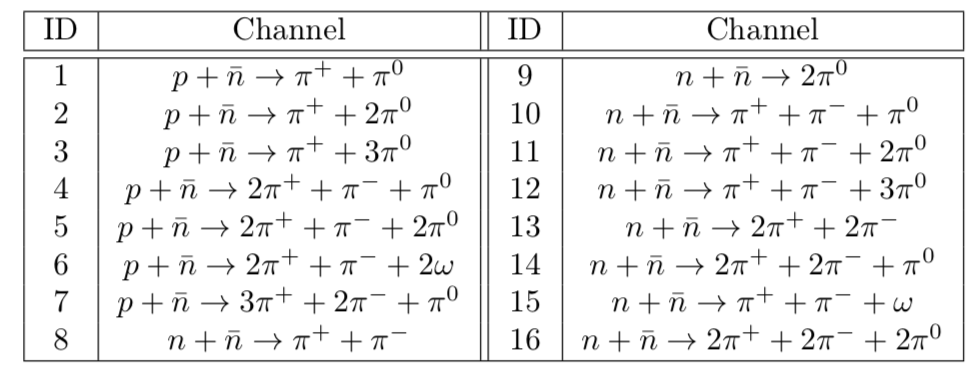
\includegraphics[width=.8\linewidth]{costas_table2}\\
    \end{centering}
  
  \caption[GENIE antineutron annihilation topologies]{Antineutron annihilation topologies considered in the GENIE neutron-antineutron oscillation simulation. TODO: replace raster version}
  \label{tbl:genie_antineutron}
\end{table}

%%%%%%%%%%%%%%%%%%%%%%%%%%%%%%%
\subsection{Detector simulation}
\label{sec:tools-mc-detsim}

%\begin{itemize}
%\item Charged particle-argon interactions
%\item Radiologicals
%\begin{itemize} \item Table from Jason Stock \end{itemize}
%\item Geometries
%\begin{itemize} \item Figure showing ProtoDUNE, 1x2x6 \end{itemize}
%\item LArG4
%\item Photon Simulation
%\begin{itemize}
%\item LAr optical properties
%\item Photon Library (or replacement) method
%\item Photon library figure
%\end{itemize}
%\item TPC detector signal simulation (Xin et al.)
%\end{itemize}

\subsubsection{LArG4}

The truth particles generated in the event generator step are passed to a {\sc geant4} v4\_10\_1\_p03 based detector simulation. In this step, each primary particle from the generator and its decay or interaction daughter particles are tracked when they traverse liquid argon. The energy deposition is converted to ionization electrons and scintillation photons. Some electrons are recombined with the positive ions~\cite{Acciarri:2013met,Amoruso:2004dy} while the rest electrons are drifted towards the wire planes. The number of electrons is further reduced due to the existence of impurities in the liquid argon, which is commonly parameterized as the electron lifetime. The default electron lifetime is 3 ms in the simulation. The longitudinal diffusion smears the arrival time of the electrons at the wires and the transverse diffusion smears the electron location among neighboring wires. More details
regarding the recent measurements of diffusion coefficients can be found
in Ref.~\cite{Li:2015rqa,ref:lar_property}.

\subsubsection{Photon Simulation}

When ionization is calculated, the amount of scintillation light is also calculated. The response of the photon detectors is simulated using a `photon library,' a pre-generated table giving the likelihood that photons produced within a voxel in the detector volume  will reach any of the photon detectors. The photon library is generated using Geant4's photon transport simulation, including 66~cm scattering length, 20-m attenuation length, and reflections off of the interior surface detectors. The library also incorporates the response vs. location of the photon detectors, capturing the attenuation between the initial conversion location of the photon and the SiPMs.

\subsubsection{TPC Detector Signal Simulation}

When ionization electrons drift through the induction wire planes toward the collection wire plane, current is induced on nearby wires. Henceforth, we refer to the induced current as a function of drift time as the field response function. 
The principle of current induction is described by the Shockley-Ramo theorem~\cite{Shockley1938,Ramo:1939vr}. For an element of ionization charge, the instantaneous induced current $i$ is proportional to the amount of drifted charge $q$: 
\begin{equation}\label{eq:shockley_ramo}
  i = - q \cdot \vec{E}_w \cdot \vec{v}_q.
\end{equation}
The proportionality factor is a product of the weighting field $\vec{E}_w$ at the location of the charge and the charge's drifting velocity $\vec{v}_q$. The weighting field $\vec{E}_w$, which depends on the geometry of the electrodes, can be calculated by removing the charge, placing the potential of the targeted electrode to the unity potential, and setting all other conductors to ground. The charge's drifting velocity $\vec{v}_q$ is a function of the external electric field, which also depends on the geometry of the electrodes as well as the applied drifting and bias voltages.

\begin{figure}[!htp]
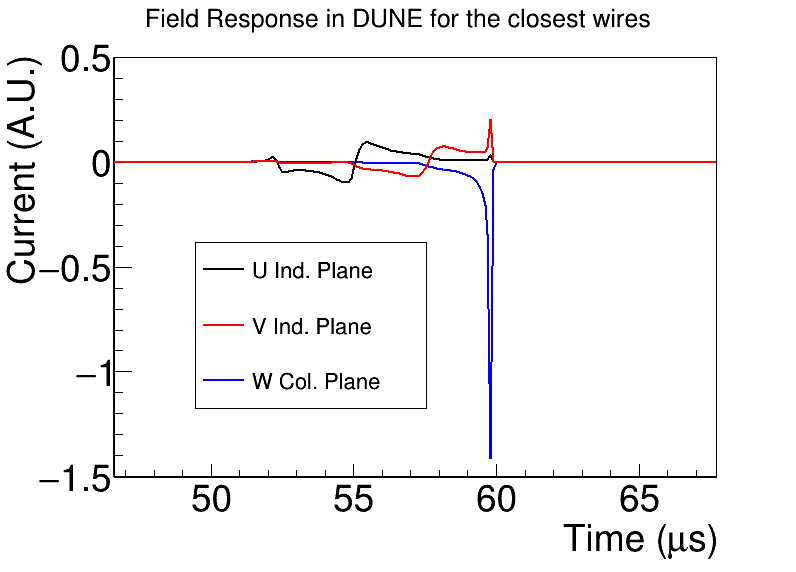
\includegraphics[width=0.7\textwidth]{field.png}
\caption[field-resp]{Field response simulated with Garfield program 
for two induction and one collection planes are shown.}
\label{field_resp}
\end{figure}

The field response functions for a single ionization electron are simulated with 2D GARFIELD~\cite{garfield}.
In the 2D GARFIELD simulation, a region with 22 cm (along the electric field or drift direction) $\times$ 30 cm (perpendicular to the field direction and wire orientation) is configured. There are five wire planes
with 5 mm spacing referred as G, U, V, Y, and M with operating bias voltages of -665 V, -370 V, 0 V, 820 V, 0 V, respectively.  These bias voltages ensure 100\% transmission of electrons through the griud plane (G) and the first two induction planes (U and V) and complete collection by the collection plane Y with the main drift field at 500 V/cm. 
  In the simulation, each wire plane contains 101 wires with 150 $\mu m$ diameter
  separating at \SI{4.73}{\mm} wire pitch. The electron drift velocity as a function of electric
  field is taken from recent measurements~\cite{Li:2015rqa,ref:lar_property}. For these
  single-electron simulation, the diffusion is turned off in the simulation. 

 Given the above GARFIELD configuration, the field response function can then be calculated
  for each individual wire in the form of induced current as a function of drift time for an
  electron starting from any arbitrary position within the region of simulation. 
  In practice, the electron is set \SI{10}{\cm} away from the wire plane above the central wire 
  The field response functions
  for $\pm$10 wires on both sides of the central wire (21 wires in total) are recorded.
  In addition to this position, five other positions with
  \SIlist{0.473;0.946;1.419;1.892;2.365}{\mm} horizontal shift towards one direction are also simulated.
  In total, 126 field responses (six positions for 21 readout wires) are calculated.
  Figure~\ref{field_resp} shows simulated field response for the closest wire for an electron starting at 
  0.473 mm horizontal shift. 
  
  In the current simulation, an average field response on the closest wire over different starting location is
  used to simulate the induced current on the wire. The induced current in the nearby wires are ignored. 
  Improvement upon this approximation is ongoing~\cite{ref:full_simulation}. 


%%%%%%%%%%%%%%%%%%%%%%%%%%%%%%%
\subsection{DAQ simulations/assumptions}
\label{sec:tools-mc-daq}

%\begin{itemize}
%\item TPC electronics and noise simulation (Xin et al.) 
%\begin{itemize} \item Signal simulation/processing figure \end{itemize}
%\item Photon detector electronics simulation
%\end{itemize}

The electrons on each wire are converted into raw wire signal (ADC vs Time) by convolution with the field response and electronics response. The ASIC electronics response was simulated with the BNL SPICE~\cite{spice} simulation.  For most samples, the ASIC gain was set to 14 mV/fC and the shaping time was set to 2 $\mu$s. For the samples generated with 3 mm wire spacing, the ASIC gain was set to 25 mV/fC. The noise level was set to 2.5 ADC RMS. In the current simulation, the electronic noise is assumed to be white, which is a uniform distribution in  the frequency domain. The implementation of a more realistic electronics noise model is ongoing. Fig.~\ref{elec_resp} shows  the expected electronics shaping functions.

\begin{figure}[!h!tbp]
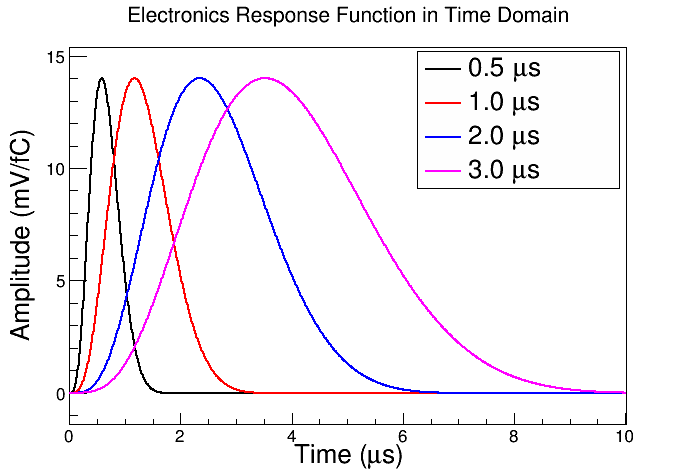
\includegraphics[width=0.7\textwidth]{elec.png}
\caption[elec-resp]{ASIC's electronics shaping functions
are shown for four shaping time settings at 14 mV/fC gain.}
\label{elec_resp}
\end{figure}


The photon detector electronics simulation separately generates waveforms 
for each channel (SiPM) of a photon detector that has been hit by photons.
Every photon that has been detected appears as a single photoelectron pulse
(with the shape taken from~\cite{http://lss.fnal.gov/archive/2015/pub/fermilab-pub-15-488-nd-ppd.pdf:2015gov}) on a randomly selected channel
(belonging to the photon detector in which the photon was registered).
Then dark noise (with the rate of $10$ Hz) and 
line noise (Gaussian noise with the RMS of $2.6$ ADC counts) are added.
Each photon (or a dark-noise pulse) has a probability of appearing
as $2$ photoelectrons on a waveform (the cross-talk probability is $16.5~\%$).
The final step of the digitization process is recording only fragments
of the full simulated waveforms that have a signal in them.
That is accomplished by passing the waveforms through a hit finder
described (See the event reconstruction)  
and storing parts of the waveforms corresponding to the hits found.


%%%%%%%%%%%%%%%%%%%%%%%%%%%%%%%%%%%%%%%%%%%%%%%%%%%%%%%%%%%%%%%%
\section{Event reconstruction in the far detector}
\label{sec:tools-fdreco}

In this section, we describe various reconstruction algorithms used to reconstruct events in the far detector TPC. %Most of them were applied to the MCC6 production.

%\begin{itemize}
%\item TPC reconstruction methods
%\begin{itemize}
%\item Demo figure for each method below
%\item TPC signal processing (Xin et al.)
%\item Hit reconstruction
%\item Track/Shower CNN
%\item TrajCluster
%\item PMA
%\item Pandora (Lorena)
%\item Wirecell (Xin et al.)
%\item SpacePointSolver
%\end{itemize}
%\item TPC Reco performance
%\begin{itemize} 
%\item Track finding efficiency vs. position, angle
%\item Shower purity/completeness comparison figures 
%\end{itemize}
%\item Photon detector reconstruction methods
%\begin{itemize}
%\item Hit finding
%\item Flash finding
%\begin{itemize} \item SN, PDK photon `event displays' \end{itemize}
%\item Calorimetry
%\end{itemize}
%\item Photon Reco Performance
%\begin{itemize}
%\item Efficiency vs. energy/position figures
%\item Timing resolution figure
%\item Energy resolution figure
%\end{itemize}
%\end{itemize}

\subsection{TPC Signal Processing}
The raw data are in the format of ADC counts as a function of TPC ticks on each wire. The signal can have a unipolar shape if it is on a collection wire or a bipolar shape if it is on an induction wire. The first step in the reconstruction is to convert the raw signal from each wire to a standard shape such as a Gaussian shape. This is achieved by passing the raw data through a calibrated deconvolution algorithm. In real detectors, excess noises may exist and need to be properly dealt with through a dedicated noise filter~\cite{Acciarri:2017sde}. There is currently no such complication in the simulation.

The deconvolution technique was introduced to LArTPC signal processing by 
Bruce Baller in the context Argoneut data analysis. The goal of 
the deconvolution~\cite{Baller:2017ugz} is to ``remove'' the impact of field and electronics responses from the 
measured signal to recover the number of ionized electrons. This technique has 
the advantages of being robust and fast and is an essential step in the overall
drifted-charge profiling process. 

Deconvolution is a mathematical technique to extract a \textit{real signal}
$S(t)$ from a \textit{measured signal} $M(t_0)$.  The measured signal is
modeled as a convolution integral over the real signal $S(t)$ and a
given detector \textit{response function} $R(t,t_0)$ which gives the
instantaneous portion of the measured signal at some time $t_0$ due to
an element of real signal at time $t$:
\begin{equation}\label{eq:decon_1}
M(t_0) = \int_{-\infty}^{\infty}  R(t,t_0) \cdot S(t) \cdot dt.
\end{equation}
If the detector response function only depends on the relative time 
difference between $t$ and $t_0$,
\begin{equation}
R(t,t_0) \equiv R(t-t_0),
\end{equation}
 we can solve the above equation by 
doing a Fourier transformation on both sides of the equation:
\begin{equation}
M(\omega) = R(\omega) \cdot S(\omega), 
\end{equation}
where $\omega$ is the frequency. In this case, we can derive the signal in the 
frequency domain by taking the ratio of measured signal and the given
response function:
\begin{equation}\label{eq:decon_2}
S(\omega) = \frac{M(\omega)}{R(\omega)}.
\end{equation}
The real signal in the time domain can then be obtained by applying the inverse Fourier 
transformation from the frequency domain. 

The response function $R(\omega)$ does not address
contributions to the measured signal which are due to real world
sources of electrical \textit{noise} from thermal and unwanted transmitting
sources or the approximation in the digitization.
Such contributions to $M(\omega)$ will not be removed by the deconvolution.
Worse, because the response function becomes small at low 
frequencies for the induction planes and at high frequencies for all
planes, the noise components in these frequencies will be
enhanced by the deconvolution.

To address the issue of noise, a \textit{filter function} $F(\omega)$ is
introduced.  Its purpose is to attenuate the problematic noise.  The
addition of this function can be considered an augmentation to the
response function.  
The two functions are kept distinct for clarity in the notation here.
Equation~\eqref{eq:decon_2} is then updated to become
\begin{equation}\label{eq:decon_filt}
S(\omega) = \frac{M(\omega)}{R(\omega)} \cdot F(\omega).
\end{equation}
With a suitable noise filtering model an improved estimator for the signal
$S(t)$ in the time domain can then be found by applying an inverse Fourier 
transform to $S(\omega)$.  Essentially, the deconvolution replaces the real field and 
electronics response function with an effective software filter response function. The 
advantage of this procedure is more pronounced on the induction plane where the irregular bipolar field response function is replaced by a regular uni-polar response function through the inclusion of the software filter. 

Since the current simulation only simulate induced current on the closest 
wire to the ionization electrons, the aforementioned 1-D deconvolution 
technique is sufficient to process the TPC signal. However, the induction 
signal in a real detector is expected to strongly depend on the local ionization charge distribution. In this case, the 1-D deconvolution is not 
enough to recover the number of ionization electrons. A 2-D deconvolution
technique, which includes both the time and wire dimensions, has been 
developed in MicroBooNE to deal with the complicated induction plane signal. Details can be found in Ref.~\cite{ref:uboone_signal_processing}. With the upcoming full TPC simulation, the 2-D deconvolution will be implemented 
in the TPC signal processing and details will be updated in the future.


\subsection{Gaussian Hit Finder}
GausHitFinder is a hit-finding algorithm that works starting from deconvolved signals on wires and defining areas above threshold known as ``pulses''. Once a pulse is found, an `n' Gaussian hypothesis is applied where `n' is defined by the number of peaks initially identified within the pulse. Based on the outcome of the fit an object known as a ``hit'' is formed and stored in the event.

\subsection{Space Point Solver}

\begin{figure}
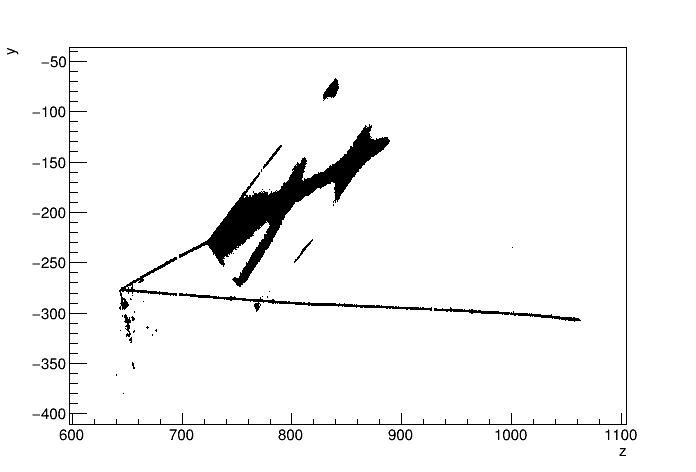
\includegraphics[width=.5\linewidth]{graphics/evd_zy_pre_2302}
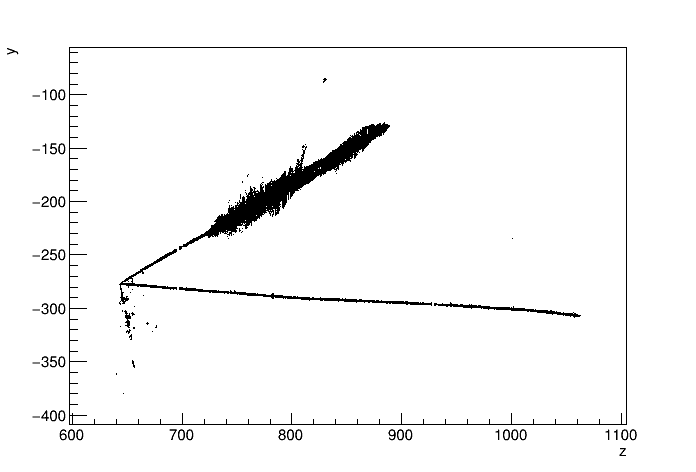
\includegraphics[width=.5\linewidth]{graphics/evd_zy_noreg_2302}\\
\makebox[.5\linewidth][c]{(a) All coincidences}
\makebox[.5\linewidth][c]{(b) Without regularization}\\
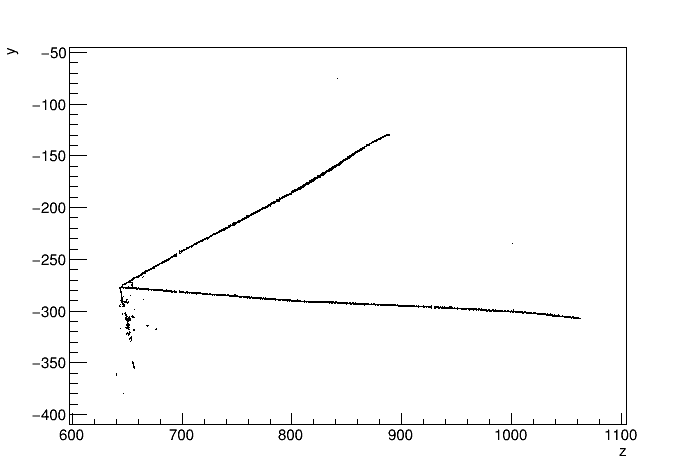
\includegraphics[width=.5\linewidth]{graphics/evd_zy_2302}
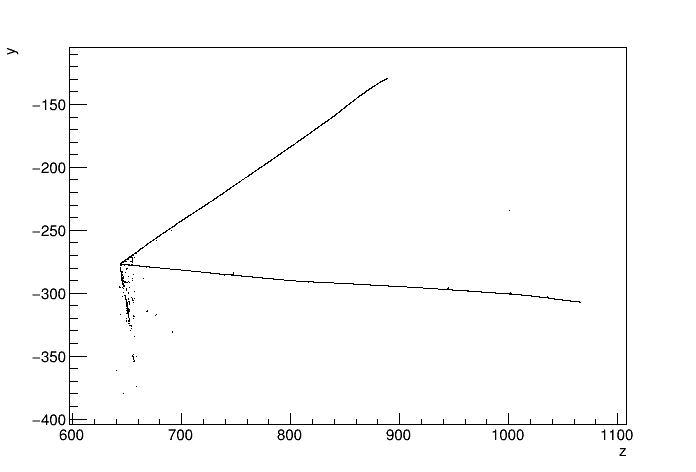
\includegraphics[width=.5\linewidth]{graphics/evd_zy_true_2302}
\makebox[.5\linewidth][c]{(c) With regularization}
\makebox[.5\linewidth][c]{(d) True charge distribution}\\

\caption[Event displays of SpacePointSolver performance]{Performance of SpacePointSolver on a simulated FD neutrino interaction. The first panel shows the position of all triplet coincidences in the $zy$ view (looking from the side of the detector), displaying multiple ambiguous regions. The second and third panels show the solution with and without regularization, the regularization disfavouring various erroneous scattered hits. The final panel shows the true charge distribution, demonstrating that the fidelity of the regularized reconstruction.}

\label{fig:spacepoint}
\end{figure}

The SpacePointSolver algorithm aims to transform the three two-dimensional views provided by the wire planes into a single collection of three-dimensional ``space points''.

First, triplets of wires are found with hits that are coincident in time within a small window (corresponding to 2mm in the drift direction) and where the crossing positions of the wires are consistent within 3.55mm\todo{check these distances}. In some cases a collection wire hit may have only a single candidate pair of induction hits and the space point can be formed immediately. Often though, there are multiple candidate triplets, for example when two tracks are overlapped as seen in one view.

SpacePointSolver resolves these ambiguities by distributing the charge from each collection wire hit between the candidate space points so as to minimize the deviations between the expected and observed charges of the induction wire hits

\begin{equation}
\chi^2 = \sum_i^{\rm wires} \left(q_i - \sum_j^{\rm points}T_{ij}p_j\right)^2
\end{equation}

where $q_i$ is the charge observed in the $i^{\rm th}$ induction hit, $p_j$ is the solved charge at space point $j$, and $T_{ij}\in\{0,1\}$ encodes whether space point $j$ is coincident in space and time with wire hit $i$.

The minimization is subject to the condition that each predicted charge $p_j\ge0$, and that the total predicted charge for each collection wire hit exactly matches observations:

\begin{equation}
\sum_j^{\rm points}U_{jk}p_j=Q_k
\end{equation}

where $Q_k$ is the charge observed on the $k^{\rm th}$ collection wire, and $U_{jk}$ encodes the coincides of space point charges with the collection wires.

The problem as formulated is convex and can thus be solved exactly in a deterministic fashion. A single extra term can be added to the expression while retaining this property:

\begin{equation}
\chi^2 \to \chi^2 - \sum_{ij}^{\rm points}V_{ij}p_ip_j .
\end{equation}

By setting $V_{ij}$ larger for neighboring points this term acts as a regularization such that solutions with a denser collection of space points are preferred. The $V$ function is chosen empirically to have an exponential fall-off with constant 2cm. %The algorithm is described more completely in \cite{spacepoint}.

Figure \ref{fig:spacepoint} shows the performance of this algorithm on a sample FD Monte Carlo event, demonstrating good performance at eliminating spurious coincidences, and the importance of the regularization term.

SpacePointSolver was developed with the intention of acting as the first stage of a fully three-dimensional reconstruction for FD neutrinos, but it has been successfully put to use in a more restricted role to solve the disambiguation problem in ProtoDUNE. The full problem is solved, but for this application the information retained is restricted to the drift volume to which the corresponding space points for each induction hit are assigned. This technique correctly resolves more than 99\% of hits while requiring less CPU time than the standard disambiguation algorithm.

\subsection{Disambiguation}
The induction wires are wrapped in the DUNE TPC design in order to save cost on electronics and minimize dead region between APAs. The consequence is that multiple induction wire segments will be read out by the same electronic channel. We need to determine which wire segment corresponds to the energy deposited by the particle in the TPC. This process is called disambiguation. 

The far detector disambiguation algorithm was originally developed for the 35t geometry. It relies on the fact that the collection wires are not wrapped and the wire angles are slightly different for the two inductions views (44.3$^{\circ}$ vs 45.7$^{\circ}$) in the 35t so that any three wires from the three planes read out by the same three channels will never cross twice. The algorithm uses gaushit as input. All the collection hits are unambiguous. Each induction hit has one channel ID and several possible wire IDs corresponding to various wire segments read out by the same channel. We need to determine which wire ID is the correct one for each induction hit. The disambiguation algorithm first loops over all collection hits. For each collection hit, it loops over all induction hits and looks for one hit on each of the two induction planes that are in time with the collection hit. Once the triplet of hits is found (one on each plane with a common time), the algorithm checks all possible wire IDs and looks for three wires that intersect. Once one and only one intersection is identified, the two induction wire IDs are assigned to the two induction hits and the ambiguation is resolved. Finally the algorithm loops over all unresolved induction hits. For each hit, it loops over all possible wire segments for that channel and chooses the wire segment that is closest to a resolved induction hit as the correct wire segment. 

The ProtoDUNE disambiguation algorithm uses the outcome of the SpacePointSolver reconstruction, which associate a 3D point with 3 hits on 3 wire planes. The 3D point can be projected onto the induction plane and the ambiguity of the induction wire signal can be resolved by choosing the wire segment that is closest to the 3D point projection. 
%(RS: protoDUNE's APAs should see signals from single TPC only)

%\subsection{Blurred Cluster}\label{sec:BlurredCluster}
%The Blurred Cluster reconstruction method aims to construct two-dimensional shower-like clusters from deposits left in the detector by showers.  It specialises in shower reconstruction, especially in the separation of nearby showers in the reconstruction of, e.g., $\pi^0$ decay.  The algorithm first applies a weighted 2D Gaussian smearing to the hit map in order to introduce `fake hits' and distribute the charge deposited in the detector more realistically.  This proceeds by convolution of a Gaussian kernel, uniquely applied for each hit given information such as rough directionality of the showering particles and the width of the reconstructed hits in time in order to introduce the most accurate blurring possible.  Clustering follows by grouping neighbouring hits within the blurred region before removing any artificial hits and forming output clusters from the remaining hit collections.  BlurredCluster uses disambiguated gaushit as input and the output clusters are in turn used as input to the EMShower algorithm (see Sec. \ref{sec:EMShower}).  More details and detailed discussion are available in Ref~\cite{ref:blurredcluster}.

\subsection{Line Cluster}\label{sec:LineCluster}
The intent of the Line Cluster algorithm is to construct two-dimensional line-like clusters using local information. The algorithm was originally known as Cluster Crawler. The ``Crawler'' name is derived from the similarity of this technique to ``gliders'' in 2D cellular automata. The concept is to construct a short line-like ``seed'' cluster of proximate hits in an area of low hit density where hit proximity is a good indication that the hits are indeed associated with each other. Additional nearby hits are attached to the leading edge of the cluster if they are similar to the hits already attached to it. The conditions are that the impact parameter between a prospective hit and the cluster projection is similar to those previously added and the hit charge is similar as well. These conditions are moderated to include high charge hits that are produced by large dE/dx fluctuations and the rapid increase in dE/dx at the end of stopping tracks while rejecting large charge hits from $\delta$-rays.
Seed clusters are formed at one end of the hit collection so that crawling in only one direction is sufficient. Line Cluster uses disambiguated gaushits as input and produces a new set of refined hits. More details on the Line Cluster algorithm can be found in Ref~\cite{ref:linecluster}.

\subsection{TrajCluster}\label{sec:TrajCluster}
TrajCluster reconstructs 2D trajectories in each plane. It incorporates elements of pattern recognition and Kalman Filter fitting. The concept is to construct a short ``seed'' trajectory of nearby hits. Additional nearby hits are attached to the leading edge of the trajectory if they are similar to the hits already attached to it. The similarity requirements use the impact parameter between the projected trajectory position and the prospective hit, the hit width and the hit charge. This process continues until a stopping condition is met such as lack of hits, an abnormally high or low charge environment, or encountering a 2D vertex or a Bragg peak.

2D vertices are found between trajectories in each plane. The set of 2D vertices is matched between planes to create 3D vertices. A search is made of the ``incomplete'' 3D vertices, those that are only matched in two planes, to identify trajectories in the third plane that were poorly reconstructed.

Two recent additions to TrajCluster are matching trajectories in 3D and tagging of shower-like trajectories. More details on the TrajCluster algorithm can be found in Ref~\cite{ref:trajcluster}.



\subsection{Pandora}\label{sec:Pandora}

The Pandora Software Development Kit~\cite{Marshall:2015rfa} was created to address the problem of identifying energy deposits from individual particles in fine-granularity detectors. It promotes the idea of a multi-algorithm approach for solving pattern-recognition problems. In this approach, the pattern recognition is broken down into a large number of decoupled algorithms, where each algorithm addresses a specific task or targets a particular topology. The overall event is then built up carefully using a chain of many tens of algorithms. The Pandora multi-algorithm approach has been applied to Liquid Argon TPC detectors, and has been successfully used in different analyses for the reconstruction of cosmic-ray muons and neutrino interactions in the MicroBooNE experiment~\cite{Acciarri:2017hat} as well as test beam interactions in the protoDUNE single phase detector~\ref{sec:performance:protodune}.


\subsubsection{Pandora Inputs and Outputs}

The Pandora pattern recognition algorithms are integrated into the LArSoft framework via the {\it larpandora} repository. The input to the pattern recognition is a list of reconstructed and disambiguated 2D hits. A ``StandardPandora'' ART Producer module translates these hits into native Pandora 2D hits, which are separated into the $U$, $V$ and $Z$ views. The hits are further separated into ``drift volumes'', defined as the regions of the detector with a common drift readout. The Producer module initiates and applies the specified chain of pattern recognition algorithms, and then outputs the results of the pattern recognition into the ART/LArSoft framework.

The output of the reconstruction is illustrated in Figure~\ref{larsoft_output}. The main output is a list of reconstructed 3D particles (termed ``PFParticles'') for each event. A PFParticle corresponds to a distinct track or shower in the event, and has associated collections of 2D hits for each view. Each PFParticle is outputted along with an associated set of reconstructed 3D positions (``Space Points''), a sequence of 3D positions and directions that describe its trajectory (``Seeds''), and a reconstructed vertex position that defines its interaction point or first energy deposit. The identity of the particle is currently not reconstructed, but PFParticles are instead characterized as track-like or shower-like according to the pattern of their hits. The topological associations between PFarticles are used to define parent/daughter relationships, which are collated into a hierarchy. A neutrino PFParticle is also created and forms the top-level parent particle in each reconstructed neutrino hierarchy.

\begin{figure}[!h!tbp]
\centering
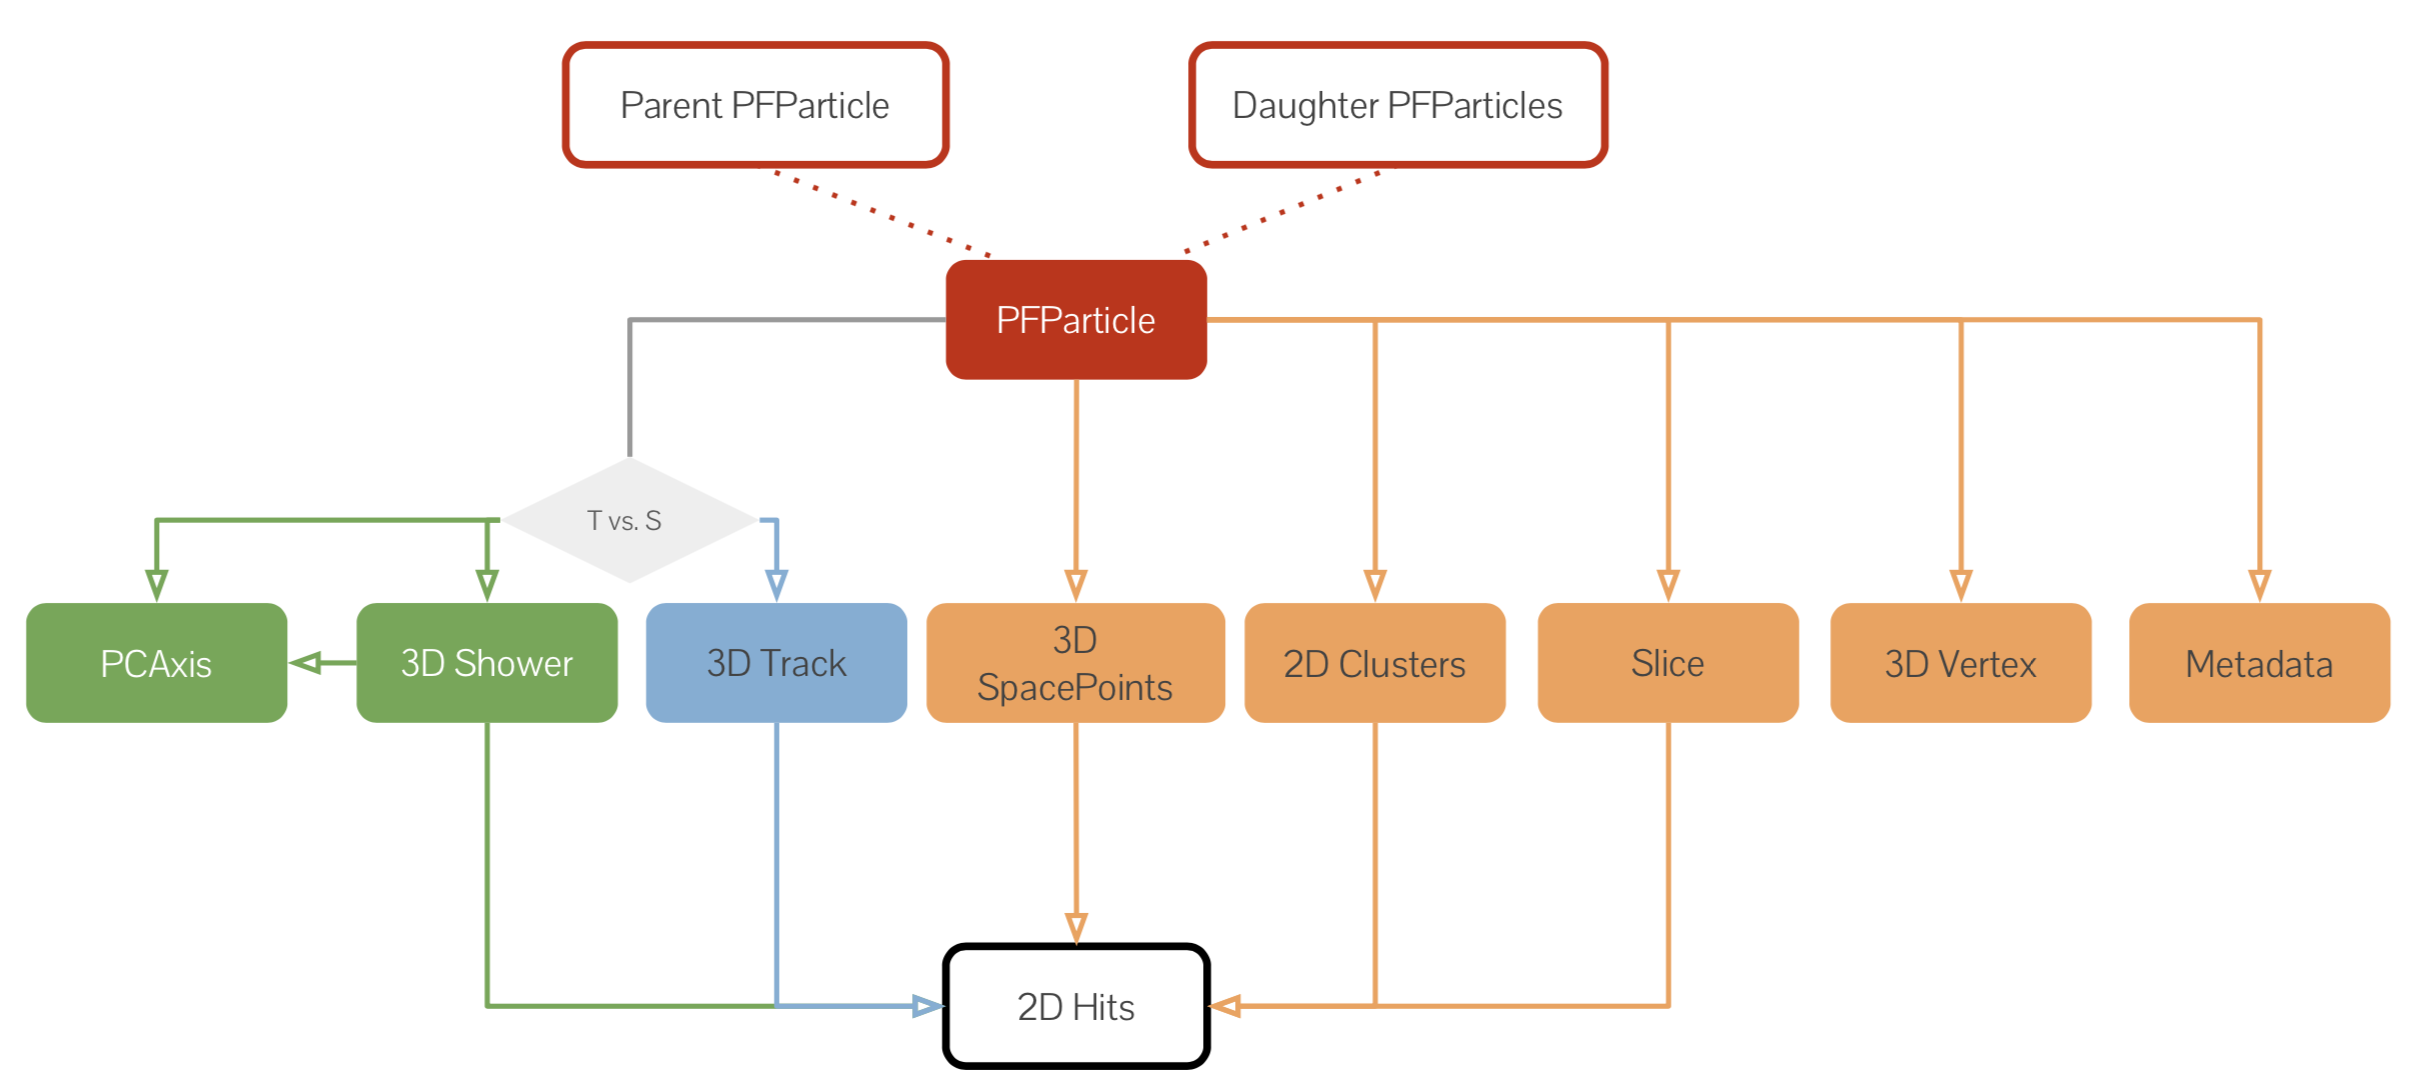
\includegraphics[width=0.8\textwidth]{FIG_LArPandoraOutputNew.png}
\caption{Illustration of the Pandora output in ART/LArSoft. Navigation along PFParticle hierarchies is achieved using the PFParticle interface, and is represented by dashed lines. Navigation from PFParticles to their associated objects is represented by solid arrows. }
\label{larsoft_output}
\end{figure}

\subsubsection{Overview of Pattern Recognition Algorithms}

The main stages of the Pandora pattern recognition chain are outlined below. Note that both the individual pattern recognition algorithms and the overall reconstruction strategy are under continual development and will evolve over time. The current chain of pattern recognition algorithms has been tuned for lower energy accelerator neutrino interactions from the Booster Neutrino Beam and is in the process of being adapted for neutrino interactions in DUNE.


\begin{enumerate}
\item{\bf 2D track-like clusters:}  The first phase of the Pandora pattern recognition is track-oriented 2D clustering. A series of topological association algorithms are used to create proto-clusters, representing continuous, unambiguous lines of 2D hits. This early clustering phase is careful to ensure that the clusters have high purity (i.e. represent energy deposits from exactly one true particle) even if this means the clusters are initially of low completeness (i.e. only contain a small fraction of the total hits within a single true particle).
\item{\bf 3D vertex reconstruction:} The vertex plays an important role in the pattern recognition. Therefore, a candidate vertex is sought at an early stage. Pairs of 2D clusters are first used to produce lists of possible 3D vertex positions. These candidate vertices are examined and scored, and the best vertex is selected.
\item{\bf 3D track reconstruction:} The aim of the 3D track reconstruction is to identify consistent track-like 2D clusters and build them into 3D track-like particles. At the same time, 3D information is used to improve the quality of the 2D reconstruction. A preliminary analysis first considers all possible combinations of 2D clusters, one from each view, and builds a rank-three tensor describing their 3D consistency between views. This tensor is then used to generate 3D particles, beginning with unambiguous combination of clusters. If there are ambiguities or inconsistencies, a series of targeted algorithms are used to identify common features in the three readout planes and iteratively correct the 2D clustering in order for unambiguous particles to emerge.
\item{\bf 2D and 3D shower reconstruction:} A series of topological metrics are first used to characterise each 2D cluster as track-like or shower-like (some use of calorimetric information would be desirable in future). An analysis of this information is then used to identify shower spines, which form the seeds for 2D and 3D shower reconstruction. A recursive algorithm is used to add shower branches onto each top-level shower spine, then branches onto branches etc. The 2D showers are then matched between views to form 3D showers.
\item{\bf 3D short track reconstruction:} Following the 3D track and shower reconstruction, a series of particle recovery algorithms are used in a number of different configurations to try and identify any remaining particles.  Many of the ideas from the earlier 3D track and shower reconstruction are re-used, but the thresholds for matching clusters between views are reduced. These algorithms take account that the particles may be missing a cluster in one view, and place particular focus on the region around the vertex.
\item{\bf 3D event-building:} This final stage of the pattern recognition begins by creating a set of 3D hits for each reconstructed particle. This 3D information is then used to organise the particles into a hierarchy of parent/daughter relationships. Each reconstructed particle is assigned a particle identification label (PDG code), depending on whether the particle was created using the 3D track reconstruction algorithms (given PDG code 13 for muons) or the 3D shower reconstruction algorithms (given PDG code 11 for electrons). An empty neutrino particle is created at the top level of the hierarchy, and assigned either PDG code 14 for numu or 12 for nue depending on whether the final-state particle with the largest number of hits is track-like or shower-like. A 3D vertex position is calculated for each of the reconstructed particles in the hierarchy, based on the point of closest approach between parent and daughter particles.
\end{enumerate}

\subsection{Projection Matching Algorithm}\label{sec:PMA}
Projection Matching Algorithm (PMA) was primarily developed as a technique of 3D reconstruction of individual particle trajectories (trajectory fit) Ref~\cite{Antonello:2012hu}. PMA was designed to address a challenging issue of transformation from a set of independently reconstructed 2D projections of objects into a 3D representation. Reconstructed 3D objects are providing also a basic physics quantities like particle directions and dE/dx evolution along the trajectories. PMA uses as its input the output from 2D pattern recognition: clusters of hits. For the purposes of DUNE reconstruction chain the Line Cluster algorithm (\ref{sec:LineCluster}) is used as input to PMA, however the use of hit clusters prepared with other algorithms may be configured as well. As a result of 2D pattern recognition, particles may be broken in 2D projections into several clusters, fractions of particles may be missing in individual projections and clusters obtained from complementary projections are not guaranteed to cover corresponding sections of trajectories. Such behavior is expected since ambiguous configurations of trajectories can be resolved only if the information from multiple 2D projections is used. Searching for the best matching combinations of clusters from all 2D projections was introduced to PMA implementation in the LArSoft framework. The algorithm attempts also to correct hit to cluster assignments using properties of 3D reconstructed objects. In this sense PMA is also a pattern recognition algorithm.

The PMA underlying idea is to build and optimize objects in 3D space (formed as polygonal lines with iteratively increased number of segments) by minimizing the cost function calculated simultaneously in all available 2D projections. The cost function consists of 2D distance of hits to the optimized object 2D projections, penalty of tracks curvature, and 3D distance of various feature points to the optimized object (used e.g. to improve performance for tracks with isochronous orientation). The track can be reconstructed using clusters from two projections while the distance of hits to the track projection in the third plane is used to validate correct association of clusters. This method is used to score 3D track candidates in the three-plane TPC configurations, like single-phase DUNE and MicroBooNE detectors and prototypes. Clusters from all planes are used in this scenario in the fine tuning of the selected candidates. In the two-plane configurations (dual-phase TPC detectors, single-phase LArIAT and ArgoNeut  detectors) the track candidates are scored by the value of cost function, which is significantly increased if the trajectory fit is being optimized to spuriously associated clusters (this is also a second-level criterion for the three-plane configurations if the validation method shows no significant difference for track candidates).


The approach of constructing entire objects in 3D allows to avoid requirement of finding associations between 2D planes on the level of individual hits. Such associations are especially problematic if several hits on a single trajectory can be found with a similar drift time value, or, if due to a low signal (or any other reason) hits are missed in one of projections. Unambiguous 3D position is calculated for each 2D hit, independently from other hits in the trajectory. Such 3D positions are more accurate than found with the ``standard'' calculation of a single 3D point using multiple 2D hits matched by drift time values, leading to the more accurate dE/dx estimation. It also allows to build 3D objects using the detector data from 2D planes directly, without an intermediate step of 3D points calculation which are subsequently used to obtain the final trajectory fit. Another advantage of the approach is capability of estimation of direction of small, few-hit tracks, or estimation of 3D PC axis of shower-like objects.

Several features were developed in LArSoft's PMA implementation in order to address detector specific issues like stitching the particle fragments found in different TPC's or an option for performing disambiguation at the 3D reconstruction stage. Since algorithms existing within the LArSoft framework or interfaced to it (see Sec. \ref{sec:Pandora}) can provide pattern reconstruction results which include the particle hierarchy description, the mode for applying PMA in order to calculate solely the trajectory fits was developed. In this mode the collections of clusters forming particles are taken from the ``upstream'' algorithm and also hit to cluster associations are not changed.


Recent developments of PMA are relying on the same principle ideas and allow to build and optimize complex structures of 3D objects, i.e. multiple particle trajectories interconnected with interaction vertices. With such approach it is possible to employ in the vertex position reconstruction the local information from several tracks simultaneously, leading also to an improved fit of each individual trajectory. The track-vertex structure is constructed after the individual trajectories are found and stitched across TPC's. Vertex candidates are found as regions of intersection of two or more tracks (including regions found beyond the track endpoints), with the threshold on the allowed region size. Tracks shorter than $nn$ cm are treated separately; they can be associated to vertex candidates found using long tracks in the first pass of the algorithm or used to create vertex candidates in the second pass. Candidates are scored by the number of intersecting tracks, and if this number is equal for two candidates the maximum angle between intersecting tracks is used select candidate and create a better defined vertex as first. The entire track-vertex structure with the newly created vertex is re-optimized using PMA principles in order to accommodate additional information in the trajectory fits. Since the new vertices may connect structures that already contain vertices, a set of rules for splitting and flipping tracks was developed to ensure that the resulting structure is always tree-like (i.e. does not contain loops). The resulting structure is described as a particle hierarchy using data products available in LArSoft.


Two important reconstruction features are currently under development in LArSoft's PMA implementation. The first is the integration of PMA input with the recognition of shower-like 2D objects (elecrtomagnetic showers, electron tracks) and track-like objects (hadron and muon tracks). Such recognition is a prerequisite of obtaining robust 3D tracking with PMA, since different fitting strategies should be applied to track and shower objects. The second feature under development is the detection of kinks and decay points missed at the 2D pattern recognition level. First attempts were made with the search for outliers in the distribution of angles in the trajectory fit. It was found that the dependence on the track orientation in 2D projection needs to be taken into account; also a potential integration with an algorithm based on 2D ADC image analysis will be explored.


%\subsection{EMShower}\label{sec:EMShower}

%mode is used when reconstructing neutrino events.The EMShower reconstruction algorithm aims to find final 3D showers and all associated properties.  It is intentionally high-level by design and relies heavily on previous reconstruction, specifically BlurredCluster (Sec. \ref{sec:BlurredCluster}) and PMA (Sec. \ref{sec:PMA}).  The reconstruction proceeds in two general steps: first, the shower objects, including all associated hits in each of the views, are found; second, the properties of these showers, such as start point, direction, energy and initial dE/dx, are determined by multiple pattern recognition and calorimetric reconstruction algorithms.

%The shower objects are created by simply matching the previously found, well-formed, shower-like clusters (provided by BlurredCluster) between the different views to form 3D objects with associated hits in each plane.  This is achieved by associating hits between the 2D shower-like clusters and 3D tracks (provided by, e.g., PMA) in order to pull together clusters from different planes into one object.  These shower hits are then analysed by various successive algorithms in order to find relevant properties before the output shower objects are constructed for later use.

%EMShower can be configured to use hits from the shower-like PFParticles identified by the Pandora package. This mode is used when reconstructing neutrino events.

%Further details and detailed discussion can be found in Ref~\cite{ref:emshower}.


\subsection{Calorimetric Energy Reconstruction and Particle Identification}

As charged particles traverse a liquid argon volume, they deposit energy through ionization and scintillation. It is important to measure the energy deposition as it provides information on particle energy and species. The algorithm for reconstructing the ionization energy in LArSoft is optimized for line-like tracks and is being extended to more complicated event topology such as showers. The algorithm takes all the hits associated with a reconstructed track. For each hit, the hit area or amplitude, in ADC counts, is converted to the charge $Q_{det}$, in fC units, on the wire using an ADC to fC conversion factor that was determined by muons or teststand measurements. To account for the charge loss along the drift due to impurities, a first correction is applied to $Q_{det}$ to get the free charge after recombination $Q_{free} = Q_{det}/e^{-t/\tau_{e}}$, where $t$ is the electron drift time for the hit and $\tau_{e}$ is the electron lifetime measured by the muons or purity monitors. The charge $Q_{\rm{free}}$ is divided by the track pitch $dx$, which is defined as wire spacing divided by the cosine of the angle between the track direction and the direction normal to the wire direction in the wire plane, to get the $dQ_{\rm{free}}/dx$ for the hit. Finally, to account for charge loss due to recombination, also known as ``charge quenching'', a second correction is applied to convert $dQ_{\rm{free}}/dx$ to $dE/dx$ based on the modified Box's model \cite{Acciarri:2013met} or the Birks's model\cite{Amoruso:2004dy}. The total energy deposition from the track is obtained by summing the $dE/dx$ from each hit: $\sum\limits_{i}^{all\ hits}(dE/dx)_{i}\cdot dx_{i}$.

If the incident particle stops in the LArTPC active volume, the energy loss, $dE/dx$, as a function of the residual range ($R$), the path length to the end point of the track, is used as a powerful method for particle identification. There are two methods in LArSoft to determine particle species using calorimetric information. The first method calculates four $\chi^{2}$ values for each track by comparing measured $dE/dx$ versus $R$ points to the proton, charged kaon, charged pion and muon hypotheses and identifies the track as the particle that gives the smallest $\chi^{2}$ value. The second method calculates the quantity $PIDA = <A_{i}> = <(dE/dx)_{i}R_{i}^{0.42}>$ \cite{Acciarri:2013met}, which is defined to be the average of $A_{i} = (dE/dx)_{i}R_{i}^{0.42}$ over all track points where the residual range $R_{i}$ is less than 30 cm. The particle species can be determined by making a selection on the $PIDA$ value. 

Figure~\ref{dedx} shows the $dE/dx$ versus residual range and $PIDA$ distributions for reconstructed $K^{+}$, $\mu^{+}$ and $e^{+}$ tracks in proton decay events. The calorimetry information is very efficient in separating those three different particles.

\begin{figure}[!ht]
\subfloat[$K^{+}$]{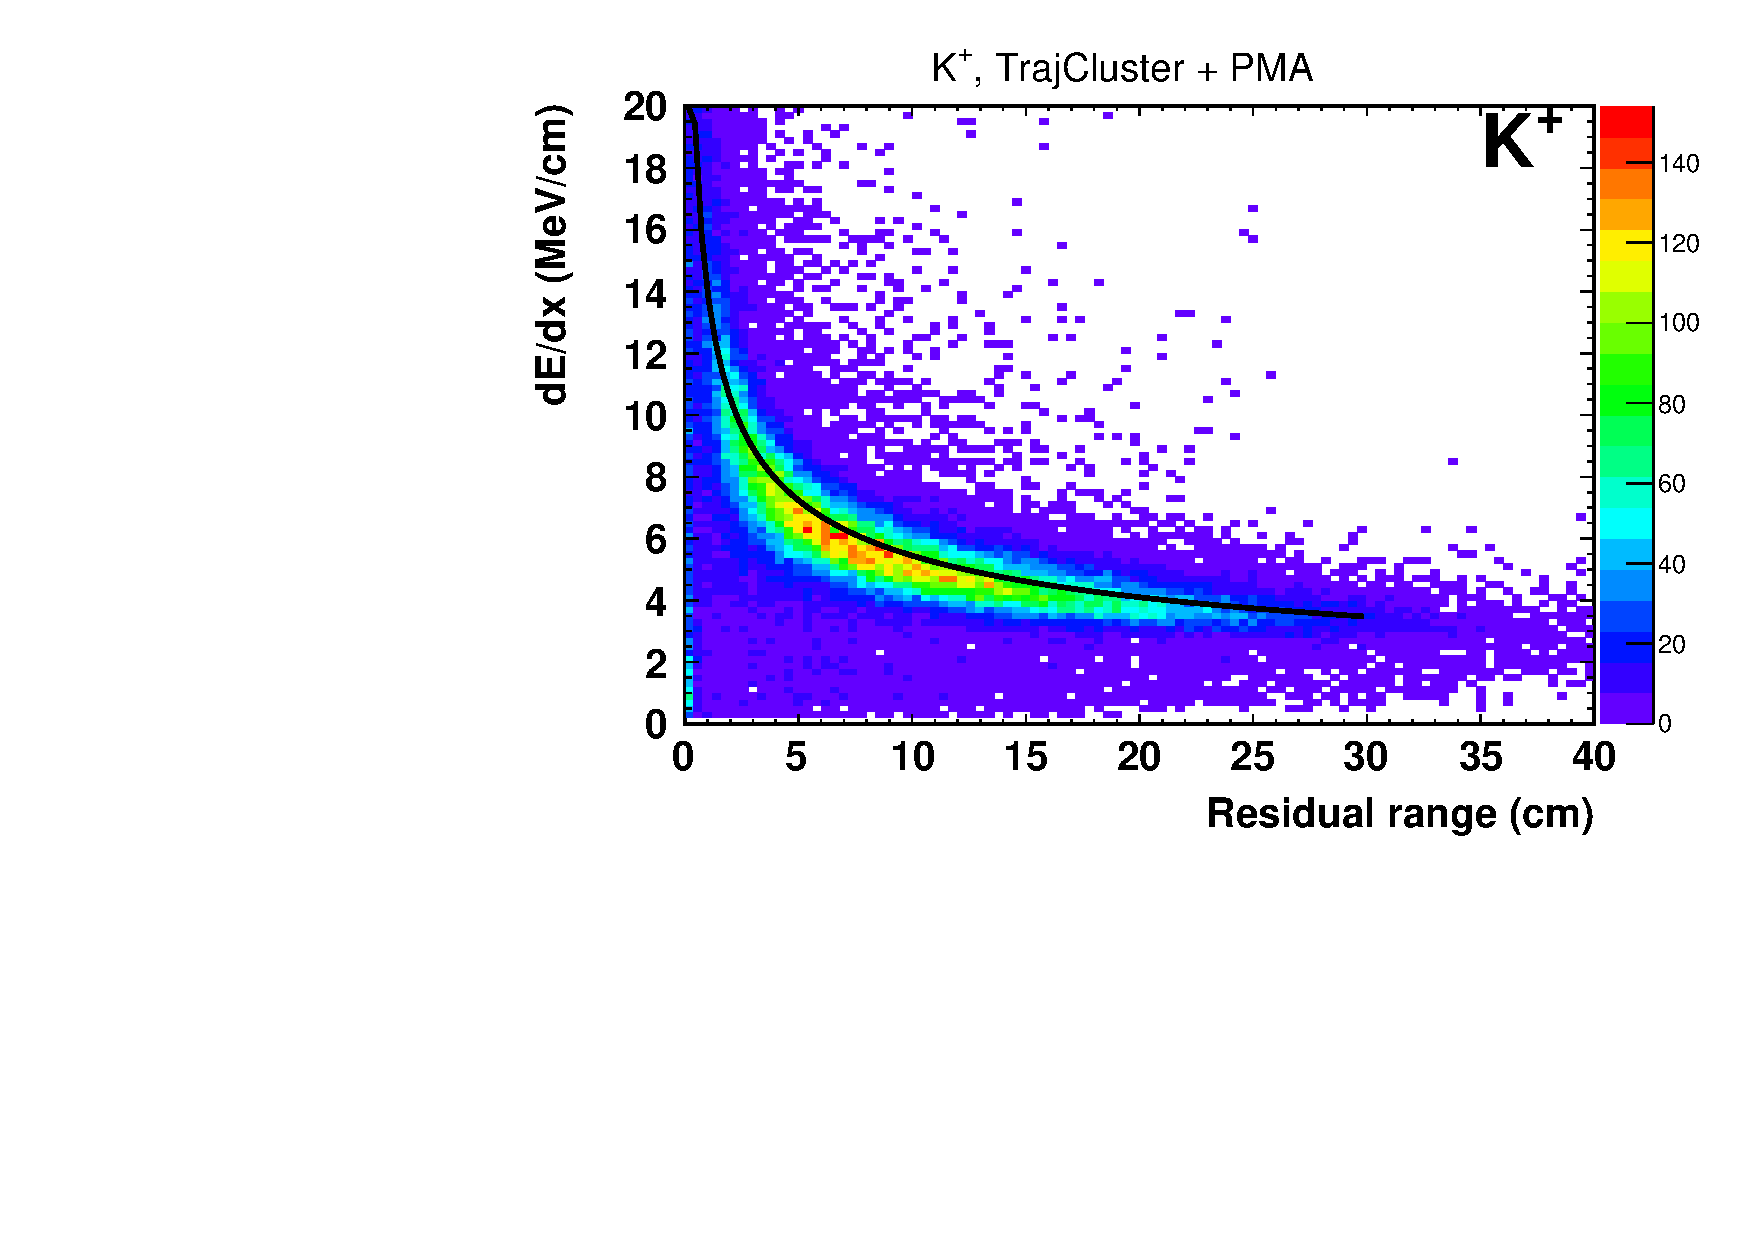
\includegraphics[width=0.5\textwidth]{dedxktc.pdf}}
\subfloat[$\mu^{+}$]{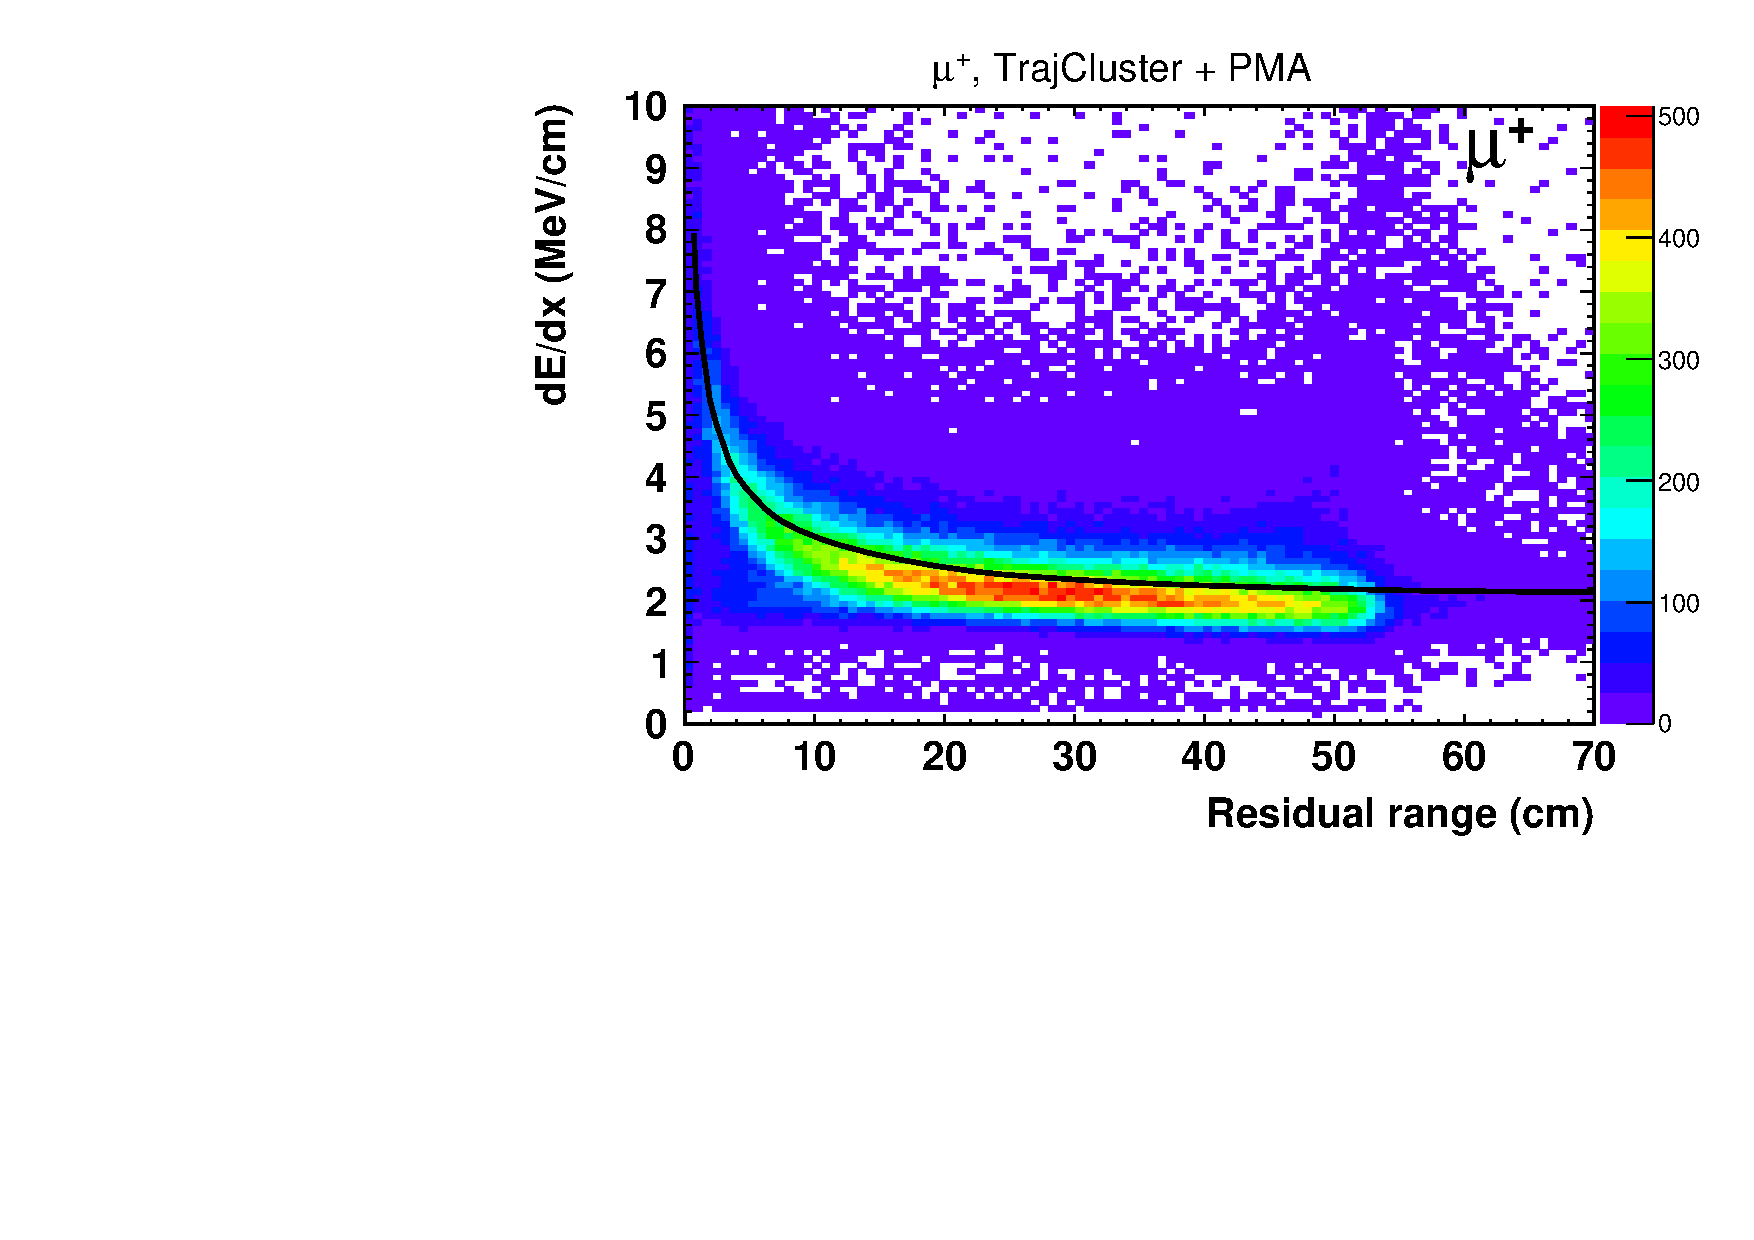
\includegraphics[width=0.5\textwidth]{dedxmutc.pdf}}\\
\subfloat[$e^{+}$]{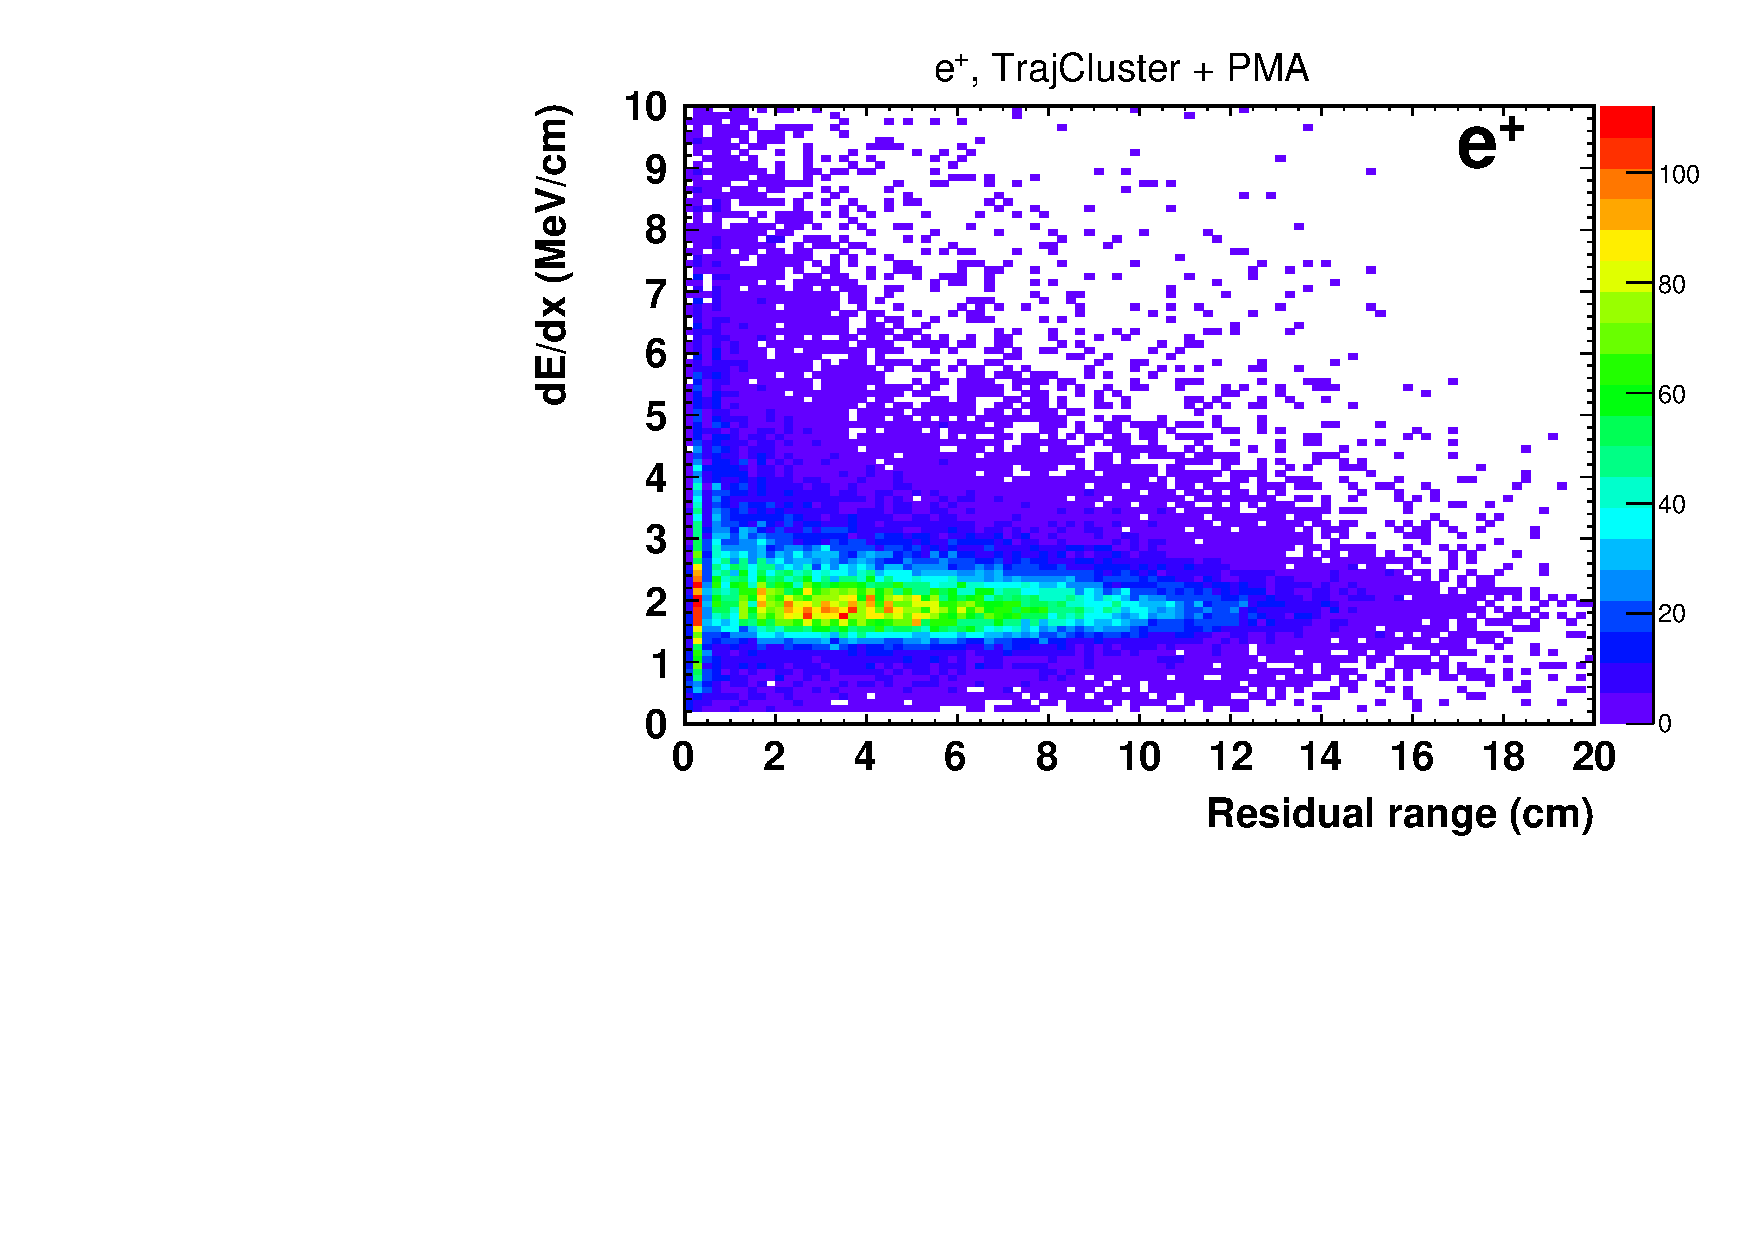
\includegraphics[width=0.5\textwidth]{dedxetc.pdf}}
\subfloat[$PIDA$]{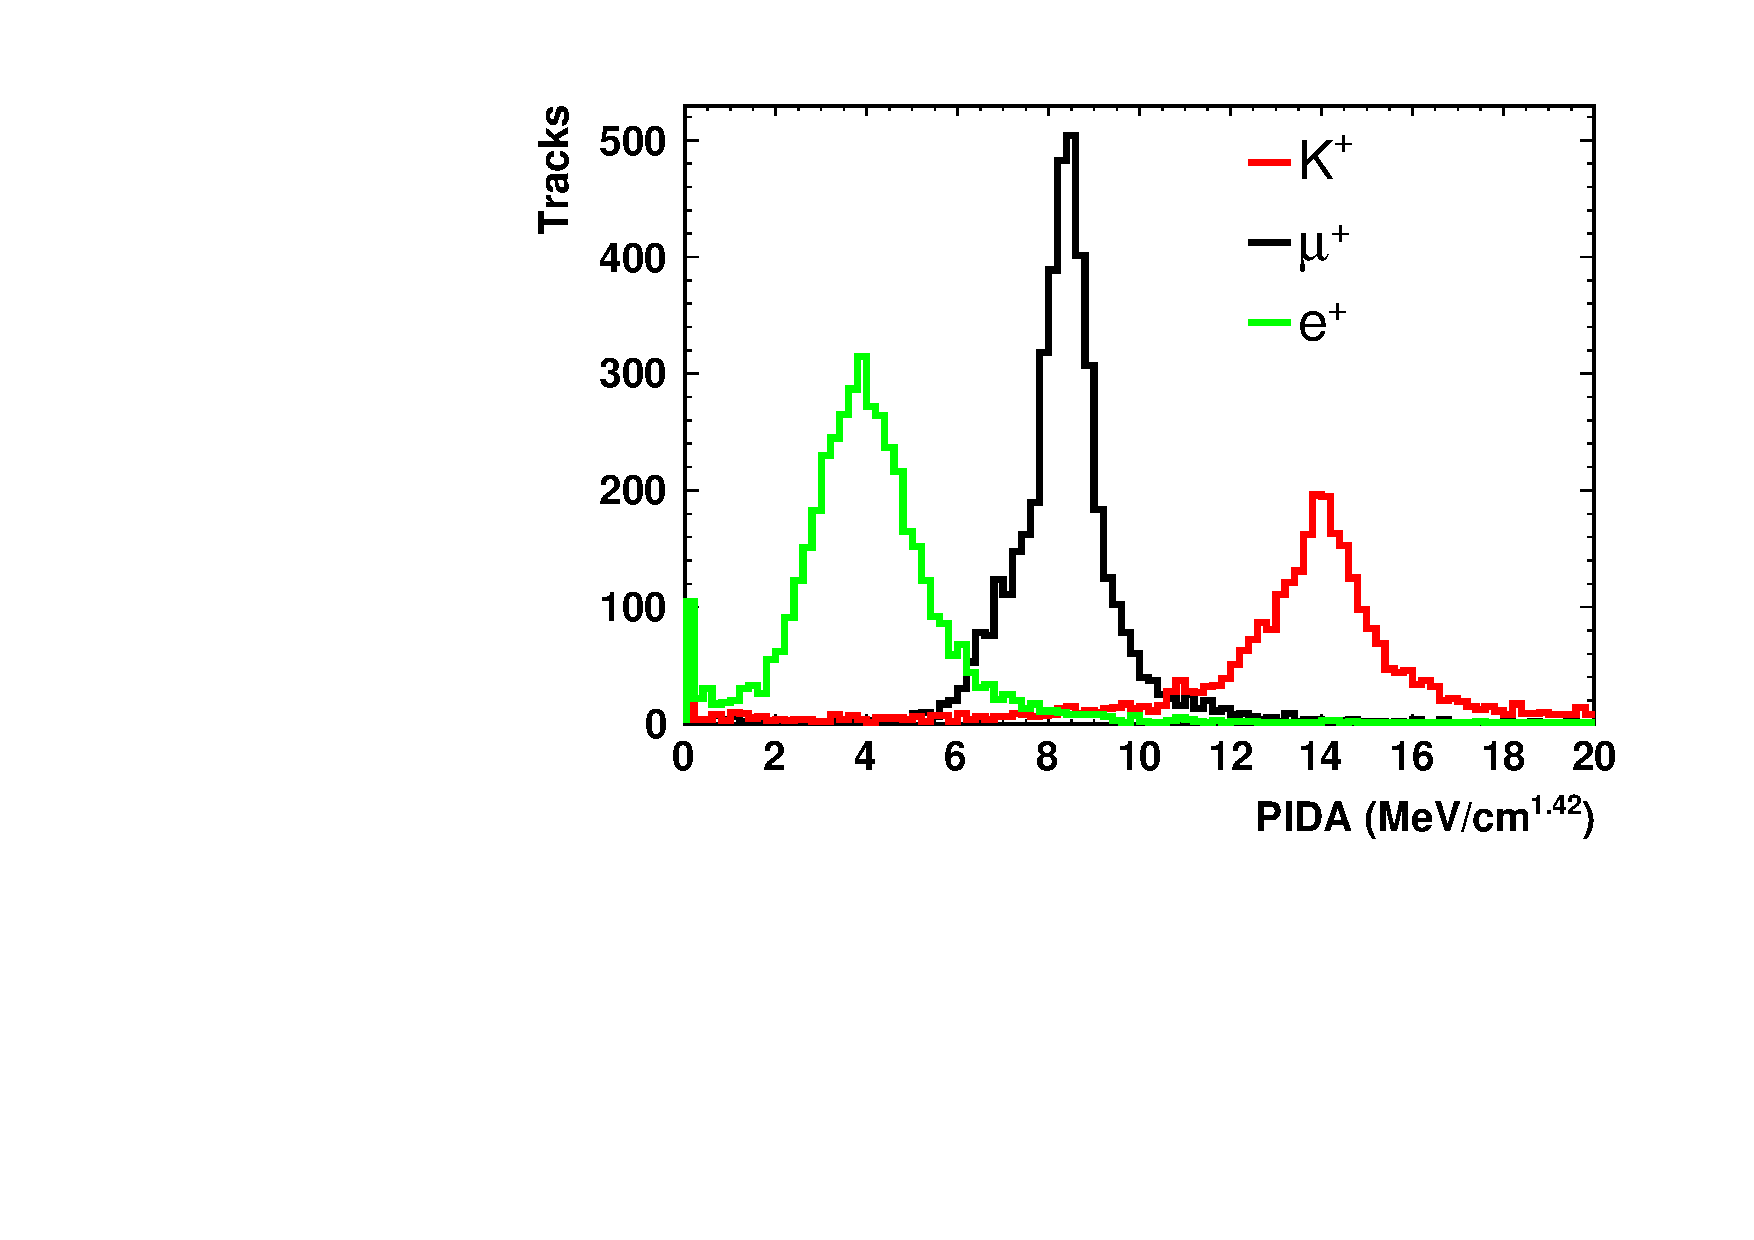
\includegraphics[width=0.5\textwidth]{pidakmue.pdf}}
\caption{(a)(b)(c): $dE/dx$ as a function of the residual range for reconstructed $K^{+}$, $\mu^{+}$ and $e^{+}$ tracks in proton decay events ($p\rightarrow\bar{\nu}K^{+}$, $K^{+}\rightarrow\mu^{+}\rightarrow e^{+}$). The black curves are theoretical predictions. (d): $PIDA$ distributions of the reconstructed $K^{+}$, $\mu^{+}$ and $e^{+}$ tracks.}
\label{dedx}
\end{figure}


\subsection{WireCell}
WireCell~\cite{wirecell}, which adopts a very different approach from the 
fore-mentioned algorithms, is a new reconstruction method under development.
Instead of directly doing pattern recognition on each of the 2D views (drift 
time vs. wire number), the first step of the WireCell reconstruction is to 
perform 3D imaging with time, geometry, and charge information. The definition
of "Hit" is based on signal strength after charge extraction in a 2 $\mu$s time slice. The usage of 
time information means that hits from different wire planes at different time 
slice cannot be associated. The usage of geometry information means that hits
from wires that are not crossing each other cannot be associated together. 
The usage of charge information means that the hits from different wire plane
with different signal strength are unlikely to be associated together. The 
usage of the charge information is quite unique for LArTPC, as each of the 
wire plane in principle detect the same amount of the ionization electrons. 
Figure~\ref{quality} shows the performance of the WireCell 3D imaging. 
The large blue blob reflects the ambiguities due to wire readout for a track
traveling parallel to the wire plane. (The 3D web-based 
display can be found at 
\url{http://www.phy.bnl.gov/wire-cell/bee/set/6/event/20/}.) In this case, a group of wires from each 
wire plane is fired simultaneously. Therefore, the time and geometry 
information will provide rather limited constraints on the hit associations. 
The advantage of the WireCell approach is that it utilizes full TPC 
information. The strong requirement of the time/geometry/charge information
provides a natural way to suppress electronic noise at the cost of more
sensitive to the hit inefficiency. Since the track and shower hypotheses
are not used, the 3D imaging works for any event topology. Once the 3D
images are reconstructed, 3D pattern recognition is needed to identify 
the content inside the image. Figure~\ref{tracking2} shows the 
performance of the current available 3D pattern recognition inside
WireCell. More developments on the WireCell pattern recognition 
are needed before the calculating of physics quantities. At the moment, the 
development of wirecell lies on the improvement in the TPC signal 
processing as well as the 3D pattern recognition techniques.


%% Wire-Cell Imaging
\begin{figure}[!ht]
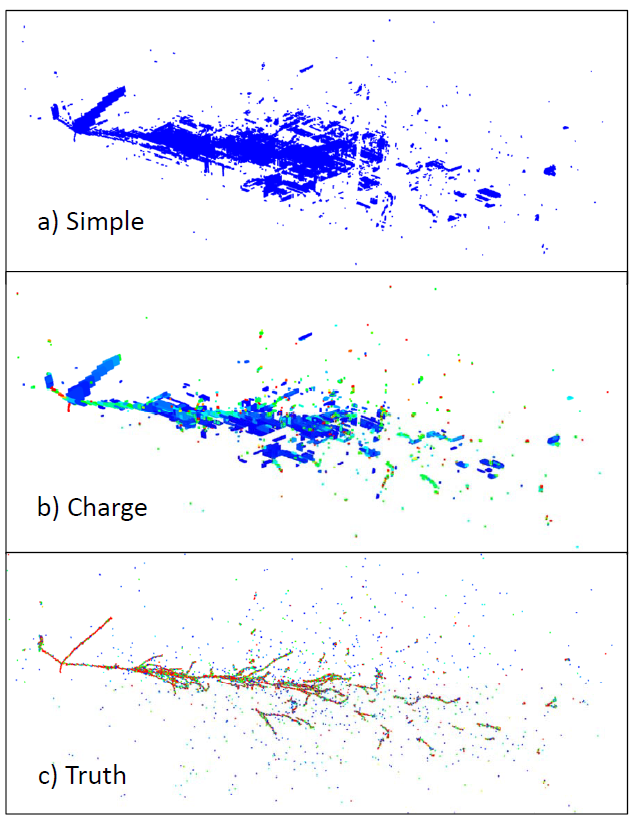
\includegraphics[width=0.8\textwidth]{quality.png}
\caption[Comparison of imaging recon
qualities with and without charge information]{Comparison of imaging reconstruction 
qualities with and without the charge information. }
\label{quality}
\end{figure}


%% Wire-Cell 3D pattern recognition
\begin{figure}[!ht]
 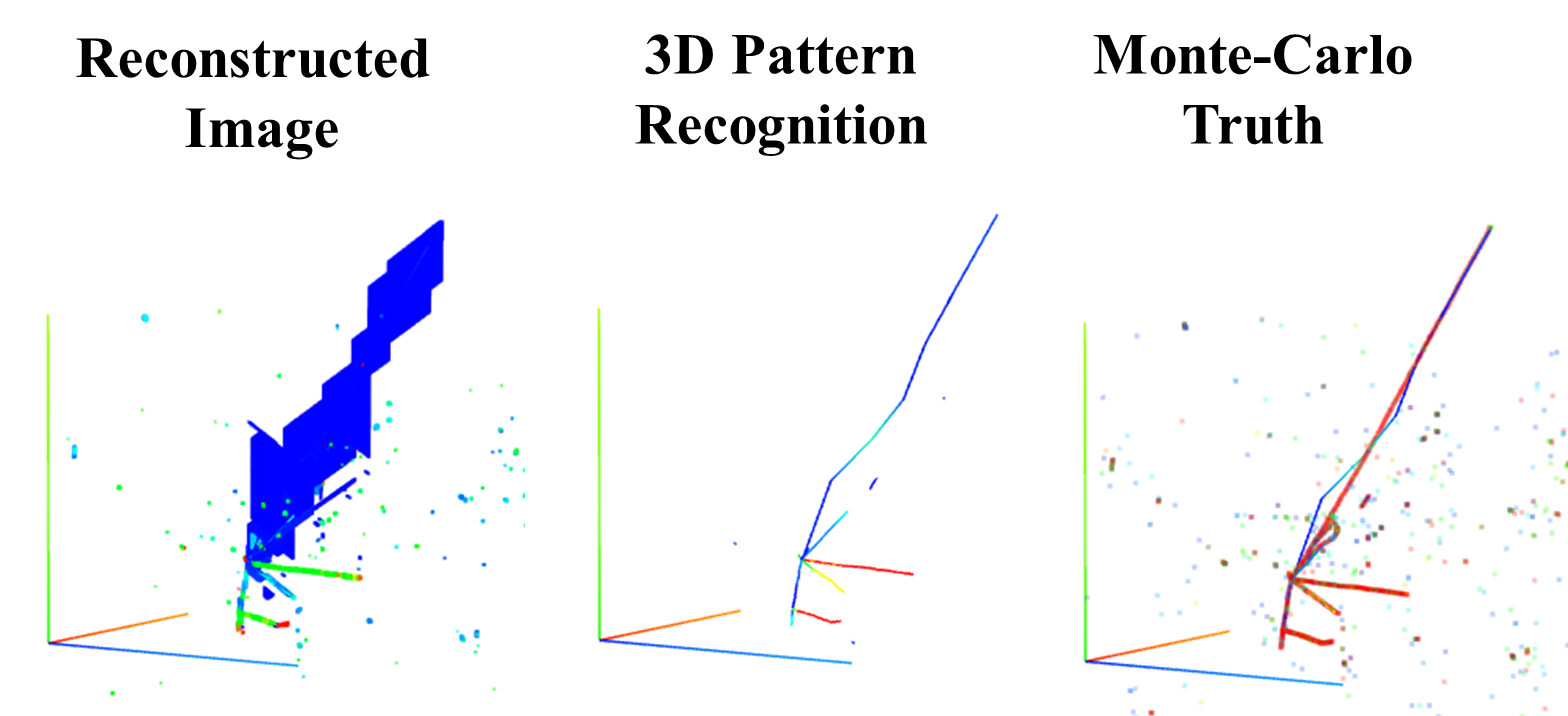
\includegraphics[width=0.96\textwidth]{Tracking_2.png}
\caption[Reconstructed image for one neutrino interaction event; comparison to MC]{The reconstructed image is shown 
on the left panel for one neutrino interaction event. The image 
was passed through the 3D pattern recognition program with tracks 
identified (middle panel). The identified pattern is compared 
with Monte-Carlo truth (right panel).}
\label{tracking2}
\end{figure}


In the following, we briefly describe the concept of Wire-Cell tomographic imaging step.
Calibrated Wire-Cell imaging determines the likely spatial distribution of
activity in the detector volume which is consistent with the measured
signals.  The distribution is defined on a collection of voxels
filling the volume.  The voxels are shaped as polygonal, right-angled
extrusions.  The two polygonal faces are called ``cells'' and are
parallel to the wire planes.

A cell covers the region near a triple-overlap of one wire from each
plane.  If one imagines a strip with width $\pm\frac{1}{2}$ wire pitch
which runs parallel to the wire and in the wire plane and then further
imagines three strips, one from a wire in each plane, overlapping then
their intersection forms a cell.

The sides of the voxels are parallel to the drift and extend to cover
the distance electrons will drift during one ``time slice'' (chosen to be four
time ticks due to expected timing resolution.).

The measured signal on a wire is subject to a threshold.  For a given
time slice, if the signal is above this threshold the wire is
considered ``hit''.  Likewise, for each time slice, any cell which has
its three associated wires ``hit'' is itself considered
``hit''.~\footnote{In the real world case where some channels do not
  read out, the signal the requirement is relaxed to consider the cell
  hit if at least two wires are hit and the third wire is a known dead 
channel.  This leads to complications such
  as producing artificial cell hits (``ghosting'').}  Given the time
of the hit cell and external information about the initial interaction
time (from the optical detector system), the cell can be projected
into the detector volume along the drift path to provide the location
of the voxel.

One of the unique features of the LArTPC is that each wire plane, be it induction or 
collection provides a measure of the same distribution of ionization electrons.
This 
feature is independent of the initial event topology (i.e. track angle, shower, vertex etc.). 
Therefore, this feature can be used to remove ambiguities made by using wire planes for the 
readout. Using the concept of wire and cell, we can thus write down the following charge 
equation:
\begin{equation}\label{eq:charge}
B\cdot W = G\cdot C.
\end{equation}
Here, $W$ represents a vector of charge measures in wires from all wire planes in a given time slice. 
$B$ is a matrix connecting \textit{merged wires} with single wires~\footnote{A group of ``merged wires'' is formed by collecting together all neighboring hit wires in the time slice.  This is done to reduce the rank of the matrix equation.}.
$C$ is a vector representing the likely amount of ionization electrons in \textit{merged cells} or \textit{blobs}~\footnote{``A group of ``merged cells'' is formed by collecting together all primitive cells which are hit and self-contiguous.}.  $G$ is the geometry 
matrix connecting merged cells and the merged wires. This equation can be expanded into 
a chi-square function:
\begin{equation}\label{eq:chi2}
\chi^2 = \left( B\cdot W - G\cdot C \right)^T V_{BW}^{-1} \left(B\cdot W - G\cdot C\right),
\end{equation}
which also takes into account the uncertainties of the measured charge in 
wires. In particular, $V_{BW} \equiv B \cdot V_{W} \cdot B^{T}$ is the 
covariance matrix describing the uncertainty in (merged) wire 
charges. 

The minimum of the above chi-square function can be found by calculating the 
first derivative
\begin{equation}
\frac{\partial \chi^2}{\partial C} = 0  \rightarrow
G^{T} V_{BW}^{-1} \left(B\cdot W - G\cdot C\right) +
\left(B\cdot W- G\cdot C\right)^{T} V_{BW}^{-1} G = 0,
\end{equation}
and the solution can be written as:
\begin{equation}\label{eq:solution}
C = \left( G^{T} \cdot V_{BW}^{-1} \cdot G \right)^{-1} \cdot G^{T} \cdot V_{BW}^{-1} \cdot B\cdot W.
\end{equation}
The core of the Eq.~\eqref{eq:solution} is the inversion of the matrix 
$G^{T} \cdot V_{BW}^{-1} \cdot G$, which will be referred to as $M$. 
When this matrix can be inverted, the charge
of merged cells can be derived directly. For faked hits (merged cells without 
any ionization charge), the derived charge is likely to be close to zero. For 
real hits (merged cells with ionization charge), the derived charge is like to be
large and close to the actual true value. On the other hand, if this matrix can not be
inverted, additional assumptions and more advanced techniques are needed to 
derive the solution. The details of these techniques are beyond the current scope of 
technote, and will be added in the future.



\subsection{Optical Reconstruction}

\subsubsection{Optical Hit Finder}
\label{sec:OpticalHitFinder}
The first step of the DUNE optical reconstruction is reading
individual waveforms from the simulated photon-detector electronics
and finding optical hits -- regions of the waveforms containing pulses.
The optical hit contains the optical channel (SiPM) that the hit
was found on, time corresponding to the hit, its width,
area, amplitude, and number of photoelectrons.

The current DUNE optical-hit-finder algorithm searches for regions of the waveform
exceeding a certain threshold ($13$ ADC counts), checking whether that region
is wider than $10$ optical TDC ticks, and, if it is, calculating the aforementioned
optical-hit parameters for the region (including parts of the waveform around it
that have ADC values greater than $1$) and recording it as an optical hit.
The number of photoelectrons is calculated by dividing the full area of the hit
by the area of a single-photoelectron pulse.
The pedestal is assumed to be constant and is specified in the hit finder as $1500$ ADC counts.


\subsubsection{Optical Flash Finder}
After optical hits are reconstructed, they are grouped into higher-level objects called optical flashes.
The optical flash contains the time and time width of the flash,
its approximate Y and Z coordinates (and spatial widths along those axes),
its location and size in the wire planes,
the distribution of photoelectrons across all photon detectors,
and the total number of photoelectrons in the flash, among other parameters.

The flash-finding algorithm searches for an increase in photon-detector activity
(the number of photoelectrons) in time using information from optical hits
on all photon detectors.
When a collection of hits with the total number of photoelectrons 
greater than or equal to $2$ is found, the algorithm begins creating an optical flash.
It starts with the largest hit and adds hits from the found hit collection 
that lie closer than $0.5$ of the combined widths of the flash under construction
and the hit being added to it.
The flash is stored after no more hits can be added to it
and if it has more than $2$ photoelectrons.

The algorithm also estimates spatial parameters of the optical flash
by calculating the number-of-photoelectron-weighted mean and 
root mean square of locations of the optical hits
(defined as centers of photon detectors where those hits were detected)
contained in the flash.

%%%%%%%%%%%%%%%%%%%%%%%%%%%%%%%%%%%%%%%%%%%%%%%%%%%%%%%%%%%%%%%%
\section{Reconstruction Performance}

An automated reconstruction of the neutrino interaction events in DUNE, often complex topologies with multiple final state particles, is a significant challenge. The current chain of Pandora pattern recognition algorithms used has been tuned for neutrino interactions from the Booster Neutrino Beam, and it is in the process of being adapted for the wide range of energies of the DUNE FD. Despite this fact, and thanks to the reusability of Pandora algorithms for different single phase LAr TPC detectors, a good performance is already achieved with this first-pass pattern recognition. Significant improvements are expected though in the upcoming years with a more dedicated tune of the current algorithms, and the development of new ones, according to the necessities of DUNE. 

The following pages show the performance of Pandora reconstruction, explained in \ref{sec:Pandora:assessment}, on simulated neutrino interactions at a single phase 10kt Far Detector module for DUNE Far Detector in \ref{sec:Pandora:DUNEFD}, and on simulated and real data test beam events in the single phase prototype ProtoDUNE in \ref{sec:Pandora:ProtoDUNE}. These performances outline the baseline performance on which improvements will continue to be made in the next years. In addition, current results on high level reconstruction performance is presented in  \ref{sec:Pandora:High}.

\subsection{Pandora Performance Assessment}
\label{sec:Pandora:assessment}
The performance of the Pandora pattern recognition is assessed by matching reconstructed PFParticles to the simulated Monte Carlo Particles (MCParticles). These matches are used to evaluate the efficiency with which MCParticles are reconstructed as PFParticles, and to calculate the completeness and purity of each reconstructed PFParticle. 

The following procedure is used to match reconstructed PFParticles with simulated MCParticles:

\begin{itemize}
\item {\bf Selection of MCParticles:} The full hierarchy of true particles is extracted from the simulated neutrino interaction. A list of ``target'' particles is then compiled by navigating through this hierarchy and selecting the final-state ``visible'' particles (allowed to be: $e^{\pm}$, $\mu^{\pm}$, $\gamma$, $\pi^{\pm}$, $\kappa^{\pm}$, $p$). Any downstream daughter particles are folded in these target particles.
\item {\bf Matching of Reconstructed 2D Hits to MCParticles:} Each reconstructed 2D hit is matched to the target MCParticle responsible for depositing the most energy within the region of space covered by the hit. The collection of 2D hits matched to each target MCParticle is known as its ``true hits''.
\item {\bf Matching of MCParticles to reconstructed PFParticles:} The reconstructed PFParticles are matched to target MCParticles by analysing their shared 2D hits. A PFParticle and MCParticle will be matched if the MCParticle contributes the most hits to the PFParticle, and if the PFParticle contains the the largest collection of hits from the MCParticle. The matching procedure is iterative, such that once each set of matched particles has been identified, these PFParticles and MCParticles are removed from consideration when making the next set of matches. 
\end{itemize}

Using the output of this matching scheme, the following performance metrics can be calculated:

\begin{itemize}
\item{\bf Efficiency:} Fraction of MCParticles with a matched PFParticle.
\item{\bf Completeness:} The fraction of 2D hits in a MCParticle that are shared with its matched reconstructed PFParticle.
\item{\bf Purity:} The fraction of 2D hits in a PFParticle that are shared with its matched MCParticle.
\end{itemize}

\subsection{Reconstruction Performance in DUNE Far Detector}
\label{sec:Pandora:DUNEFD}

The performance of the Pandora pattern recognition has been evaluated using a sample of accelerator neutrino interactions simulated using the reference DUNE neutrino energy spectrum and the 10\,kton Far Detector geometry. The following plots show that a good efficiency is already achieved, and indicate as well particular regions and channels in which improvements can be made. 

\begin{figure}[!ht]
\centering
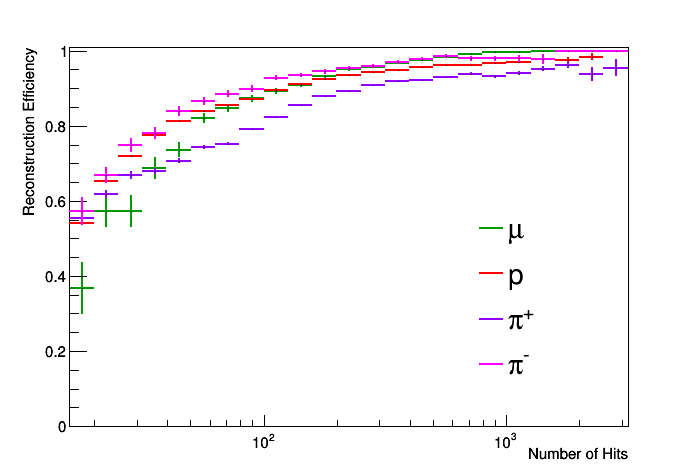
\includegraphics[width=0.5\textwidth]{Pandora-ALL_BUT_DIS_HitsEff_Tracks.png}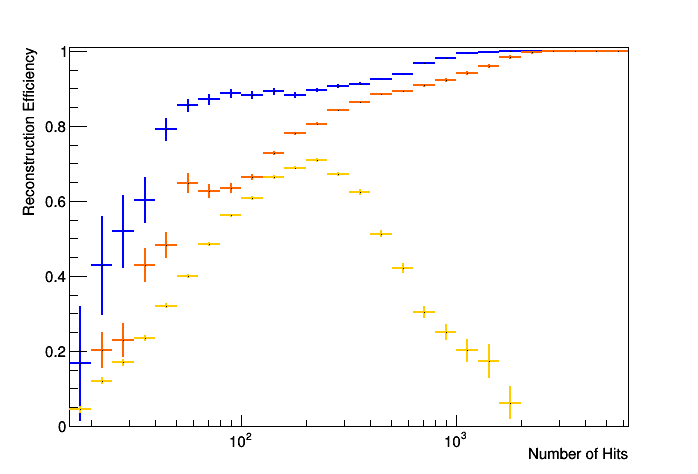
\includegraphics[width=0.5\textwidth]{Pandora-ALL_BUT_DIS_HitsEff_Showers.png}
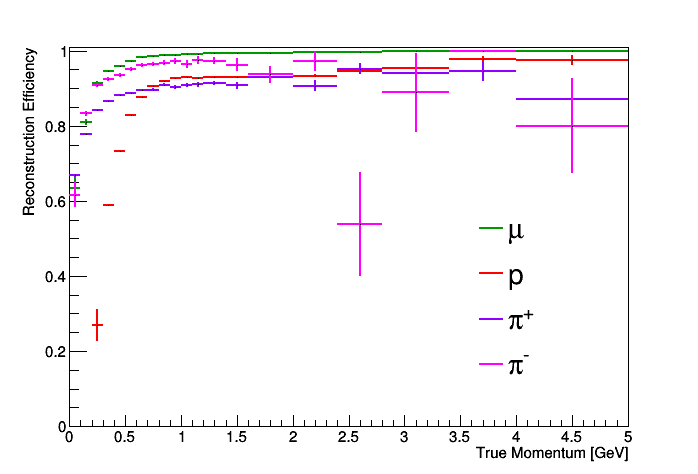
\includegraphics[width=0.5\textwidth]{Pandora-ALL_BUT_DIS_MomentumEff_Tracks.png}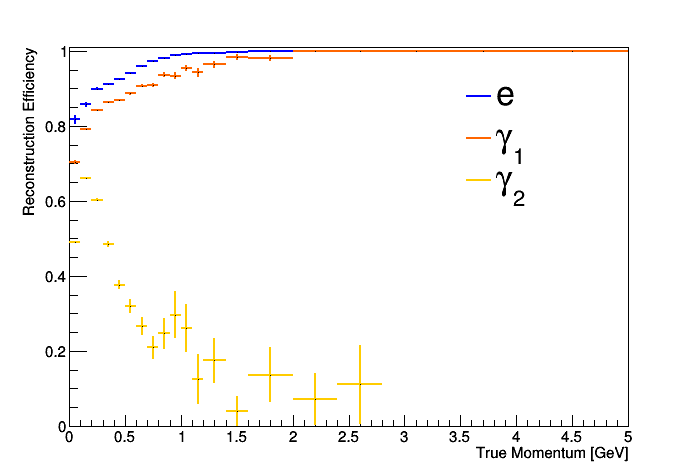
\includegraphics[width=0.5\textwidth]{Pandora-ALL_BUT_DIS_MomentumEff_Showers.png}
\caption{The reconstruction efficiency of the Pandora pattern recognition obtained for a range of final-state particles produced in all types of accelerator neutrino interactions except deep inelastic ones at DUNE FD. The efficiency is plotted as a function of the total number of 2D hits associated with the final-state MCParticles (summed across all views) on the top row, and as a function of the true momentum of the particle on the bottom row. Plots are shown for track-like particles (left) and shower-like particles (right) of each type leading in the event (in addition to the sub-leading photon $\gamma_2$ added for reference to $\pi^0$ reconstruction).}
\label{pandora_particle_efficiency}
\end{figure}

Figure~\ref{pandora_particle_efficiency} shows the reconstruction efficiency as a function of the number of total true 2D hits and as a function of the true momentum for a range of final-state particles. The typical reconstruction efficiencies obtained for track-like MCParticles ($\mu^{\pm}$, $\pi^{\pm}$, $p$) rise from 65-85\% for simulated particles depositing 100\,hits to 85-100\% for particles with 1000\,hits. The reconstruction efficiency for shower-like MCParticles ($e^{-}$,$\gamma$) is a bit lower than the equivalent for track-like particles at lower number of hits, but comparable with $>$100\,hits. The case of the sub-leading photon $\gamma_2$ is particularly challenging given the correlation with the leading one $\gamma_1$ in the $\pi^0$ decays, which may result in accidentally merging both photons; therefore a loss of efficiency is expected, and subject to improvements, for this particular channel. 

Figure~\ref{pandora_completeness_purity} shows distributions of completenesses and purities for a range of final-state particles. In the case of final-state track-like particles, a good completeness and purity are both achieved, indicating that the track-based pattern recognition algorithms currently provide a high quality reconstruction. It can be seen that final-state shower-like particles are typically reconstructed with high purities, but somewhat lower completenesses, indicating that, although the shower reconstruction is fairly good already, there is room for improvement in this particular chain of algorithms for the DUNE experiment. 

For deep inelastic interactions, in which tens of final-state particles are produced, a breakdown such as in figures~\ref{pandora_particle_efficiency} and ~\ref{pandora_completeness_purity} is more tedious and less informative. Instead, in figure~\ref{pandora_dis} we present an assessment of the reconstruction of such events by comparing the number of reconstructed particles as a function of the number of true final-state particles in the event for neutral-current (left) and charged-current (middle) deep inelastic interactions. These distributions are more populated in the diagonal, as they should be for perfect 1:1 reconstruction, indicating a good level of reconstruction of such events up to >5 final-state particles. In addition, the number of reconstructed particles matching the leading lepton in charged-current deep inelastic interactions is also presented (right), which shows a consistently predominant single match for the leading lepton. 

Figure~\ref{pandora_vertex_resolution} shows distributions of the displacements $\Delta x$, $\Delta y$ and $\Delta z$ between the reconstructed and simulated neutrino interaction positions for all types of accelerator neutrino events. It can be seen that, for the vast majority of events, the reconstructed neutrino  interaction vertex lies within $2$\,cm of the MC truth in $x$, $y$ and $z$. While the $\Delta x$ and $\Delta y$ distributions are both symmetrical and sharply peaked around the origin, a small forward bias can be seen in the $\Delta z$ distribution. The reason for this bias comes from the fact that the neutrino interaction will be boosted in the forwards Z direction, therefore being in that direction where the concentration of activity and energy depositions will appear, with vertex candidates therefore being more likely created at $\Delta z>0$ than $\Delta z<0$.  

\begin{figure}[!ht]
\centering
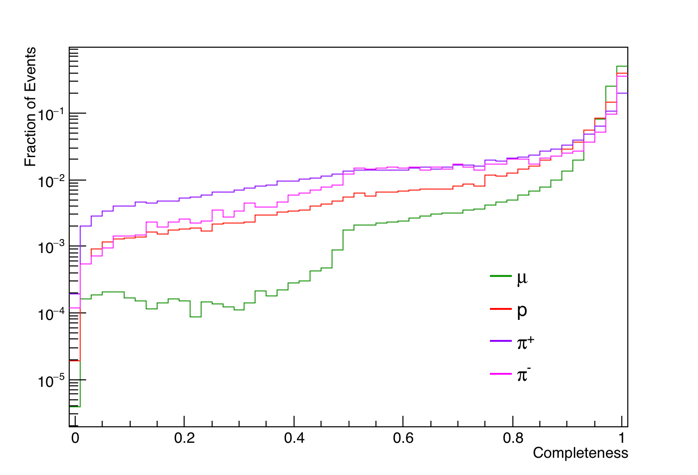
\includegraphics[width=0.5\textwidth]{Pandora-ALL_BUT_DIS_Completeness_Tracks_Log.png}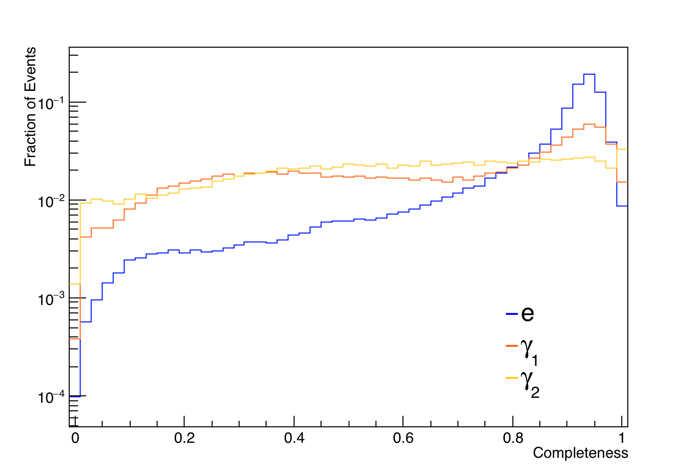
\includegraphics[width=0.5\textwidth]{Pandora-ALL_BUT_DIS_Completeness_Showers_Log.png}
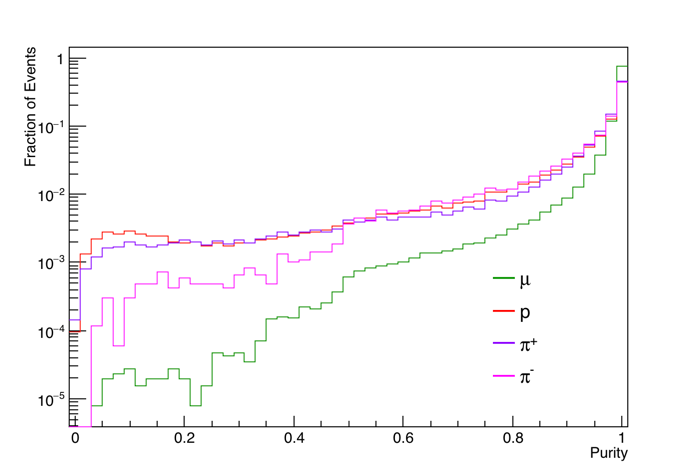
\includegraphics[width=0.5\textwidth]{Pandora-ALL_BUT_DIS_Purity_Tracks_Log.png}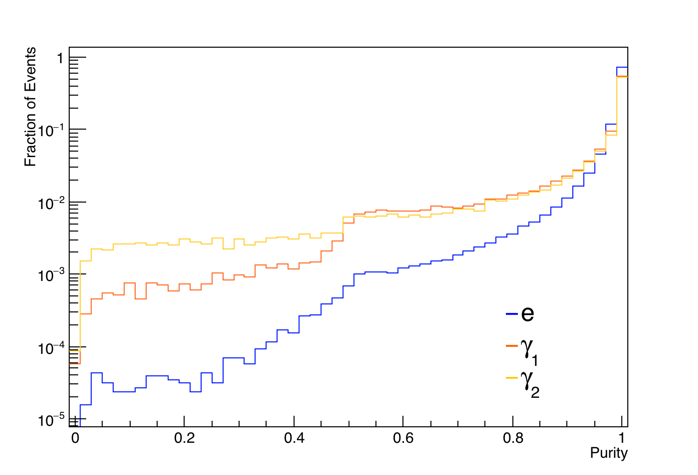
\includegraphics[width=0.5\textwidth]{Pandora-ALL_BUT_DIS_Purity_Showers_Log.png}
\caption{Distributions of completenesses (top) and purities (bottom) for a range of final-state particles divided into track-like (left) and shower-like (right), produced in all types of accelerator neutrino interactions except deep inelastic ones at DUNE FD. }
\label{pandora_completeness_purity}
\end{figure}

\begin{figure}[!ht]
\centering
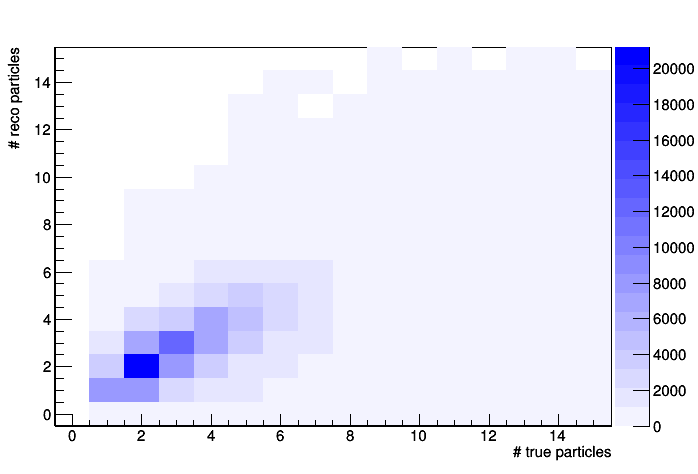
\includegraphics[width=0.35\textwidth]{Pandora-NCDIS.png}
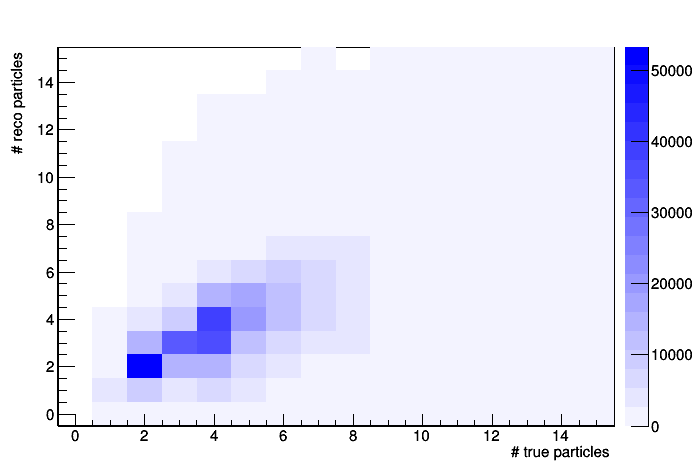
\includegraphics[width=0.35\textwidth]{Pandora-CCDIS.png}
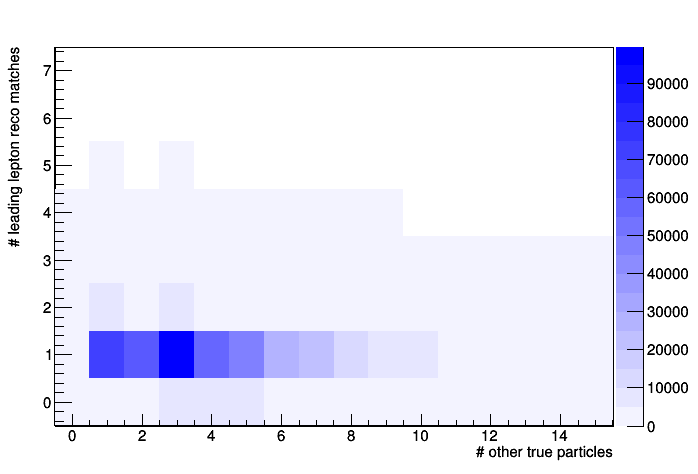
\includegraphics[width=0.35\textwidth]{Pandora-CCDISLeptonMatches.png}
\caption{Distributions of number of reconstructed particles as a function of number of true final-state particles in deep inelastic events for neutral-current (left) and charged-current (middle) interactions. In addition, the number of reconstructed particles matching the leading lepton in charged-current deep inelastic interactions is also presented (right).}
\label{pandora_dis}
\end{figure}


\begin{figure}[!ht]
\centering
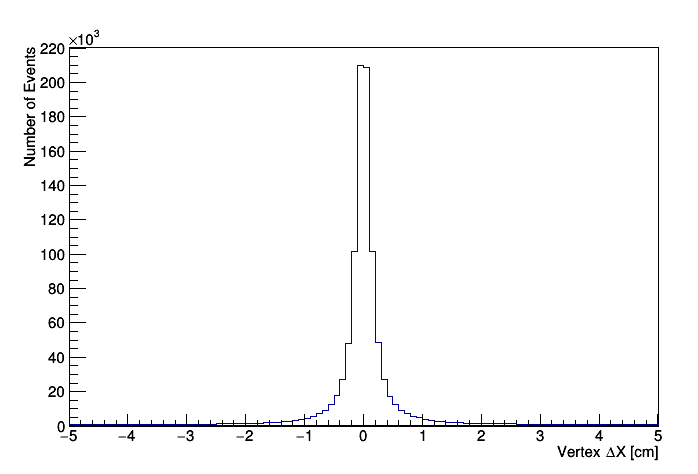
\includegraphics[width=0.35\textwidth]{Pandora-ALL_INTERACTIONS_VtxDeltaX.png}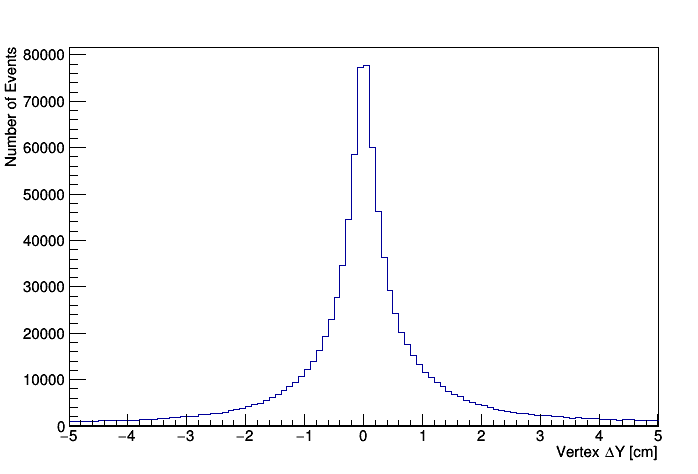
\includegraphics[width=0.35\textwidth]{Pandora-ALL_INTERACTIONS_VtxDeltaY.png}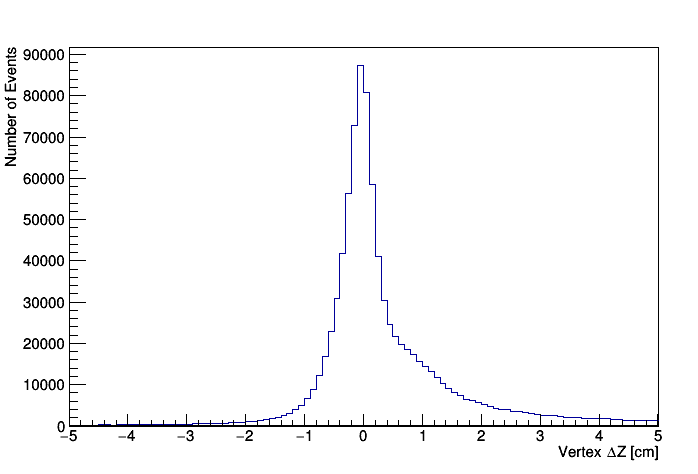
\includegraphics[width=0.35\textwidth]{Pandora-ALL_INTERACTIONS_VtxDeltaZ.png}
\caption{The displacements between the reconstructed and simulated neutrino interaction vertices. The distributions are plotted for $x$ (left), $y$ (centre) and $z$ (right) and include all types of accelerator neutrino interaction (also deep inelastic events).}
\label{pandora_vertex_resolution}
\end{figure}

\subsection{Reconstruction Performance in single phase ProtoDUNE}
\label{sec:Pandora:ProtoDUNE}


\subsection{High Level Reconstruction}
\label{sec:Pandora:High}


%%%%%%%%%%%%%%%%%%%%%%%%%%%%%%%%%%%%%%%%%%%%%%%%%%%%%%%%%%%%%%%%
\section{Tools and assumptions employed for evaluation of near detector capabilities}
\label{sec:tools-nd-eval}